\shorthandoff{"}
\chapter{Person-Environment Fit}
\label{ch:personEnvironmentFit}

\section{Einführung}
\label{ch:personEnvironmentFit:einfuehrung}
Der Person-Environment Fit ist ein Konzept in der Verhaltenspsychologie \cite[S. 1f.]{edwards:2008}. Er enthält drei zentrale Größen: Person, Umgebung (Environment) und Ergebnis (Outcome) \cite[S. 2f.]{livingstone:1997}. Forscher dieses Fachgebietes gehen davon aus, dass ein Ergebnis stets vom Zusammenspiel von Person und Umgebung abhängig ist und nicht durch eine der beiden Größen alleine bestimmt wird \cite[S. 1]{muchinsky:1987}. In der Literatur wird die Person in der Regel als menschliches Individuum interpretiert. Umgebung und Ergebnis sind dagegen breite Terminologien, welche je nach Forschungsdomäne spezifiziert werden \cite[S. 5]{edwards:2007}. Beispiele für Ergebnisse sind Zufriedenheit \cite[S. 1]{lashani:2021}, Wechselbereitschaft \cite[S. 1]{amarneh:2021}, Kreativität \cite[S. 1]{duan:2019}, Leistung \cite[S. 7f.]{elfenbein:2007} und  Berufswahl \cite[S. 1]{cable:1996}. Als Umgebung wurden in der Literatur unter anderem Unternehmen \cite[S. 1]{kristof:1996}, Gruppen \cite[S. 1]{werbel:2001} und Arbeitsplätze \cite[S. 1]{lu:2014} untersucht. Aus Person und Umgebung entsteht ein Person-Environment Fit, wenn beide Größen gleich stark ausgeprägt sind \cite[S. 53]{edwards:2008}. Der Begriff Person-Environment wird häufig als P-E Fit abgekürzt und findet sich in der Literatur auch unter ähnlichen Bezeichnungen wie Match, Ähnlichkeit, Korrespondenz oder Kongruenz.

- PE Fit ist die abhängige Variable


 (Hier Definition einfügen). Abbildung \ref{fig:personEnvironmentFit:einfuehrung:abb1} verdeutlicht, dass aus Person und Umgebung der P-E Fit entsteht. Dieser ist die abhängige Variable, welche zur Bestimmung des untersuchten Ergebnisses herangezogen wird. In der Regel führt ein stärkerer Fit zu besseren Ergebnissen. \\
\begin{figure}[h]
	\centering
	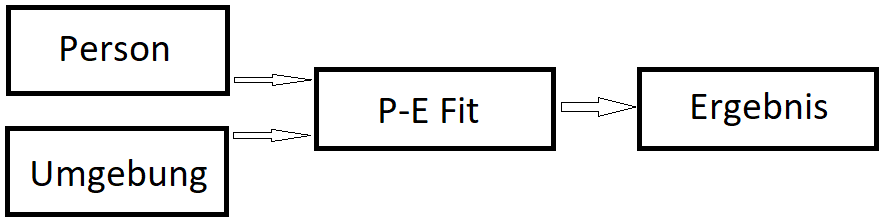
\includegraphics[width=1\textwidth]{gfx/P-E Fit.png}
	\caption{Hier eine Beschreibung einfügen und nochmal schön machen}
	\label{fig:personEnvironmentFit:einfuehrung:abb1}
\end{figure}
\\
In der Literatur wird unter dem P-E Fit meist kein Zustand, sondern ein andauernder Prozess verstanden.

- Vergleichbare Konstrukte mit vergleichbaren Dimensionen --> Wie verrechnen? --> Supplementary/Complementary

\section{Supplementary und Complementary Fit}
\label{ch:personEnvironmentFit:SupCompFit}
\newpage
https://www.sciencedirect.com/science/article/pii/S0001879115300129 \\
- Ähnlichkeit oder Kongruenz wird als Fit bezeichnet. Führt zu Outcome. Wie diese berechnet wird --> Supplementary oder Complementary

- Nadler und Tushman 1980 \\
- Rynes und Cable 2003 stellten fest, dass Bewerber das Unternehmen bevorzugen, in welchen sie am besten performen können \\
- Mortimer und Lorence 1979 stellten fest, dass die Mitgliedschaft in einer Organisation die Werte und Persönlichkeit einer Person formt \\
Prozess!!!


GRUNDLEGENDES
- \cite[S. 53]{edwards:2008}: Bedeutung des Begriffes "fit": In der Literatur werden verschiedene Begriffe Synonym für Fit verwendet, z.B. Match, Ähnlichkeit, Kongruenz zw. Person und Umgebung --> Das sind klare Begriffe, welche die Nähe von Person und Umgebung zueinander bezeichnen --> Das ist laut Edwards die richtige Konzeptualisierung für fit; Viele Autoren verwenden Begriffe ohne klare Bedeutung wie Harmonie, Kompatibilität, etc.; Fit wird auch als Interaktion oder wechselseitige Beziehung bezeichnet; Um die Bedeutung des Begriffes fit zu klären, sollten laut Edwards Begriffe verwendet werden, welche sich auf die Annäherung von P und E zu beziehen und weniger Metaphern verwenden \\
%- \cite[S. 2]{edwards:2008}: Den Grundstein für die P-E fit Forschung haben insbesondere Murrays (zwei Quellen) Need-Press-Modell und Lewins Feldtheorie (Zwei Quellen) gelegt --> Ausgehend von dieser Arbeit (meint wahrscheinlich Lewin) ist der P-E fit als ein Kernkonzept in Jobzufriedenheit, Job Stress, Berufswahl, Rekrutierung und Auswahl und Organisationskultur und Klima hervorgegangen (zu allem Quellen) --> Diese verschiedenen Strömungen haben hunderte Studien generiert, die in Zusammenfassungen (Quellen) und Meta-Analysen (Quellen) gereviewed wurden \\
- \cite[S. 3]{su:2015}: Alle P-E fit Theorien teilen die folgende Annahme: Menschen suchen und erstellen Umgebungen, die es ihnen erlauben, durch ihr Verhalten ihre Charaktereigenschaften zu manifestieren (z.B. suchen dominante Personen Leitungsfunktionen); Das Ausmaß, zu dem Menschen in ihre Arbeitsumgebungen passen (fit), hat signifikante Auswirkungen (z.B. Zufriedenheit, Performance, Stress, etc.) --> Umso besser der fit umso besser die Ergebnisse \\
- \cite[S. 3]{su:2015}: P-E fit ist ein wechselseitiger und andauernder Prozess, bei dem Leute ihre Umgebung formen und die Umgebung die Leute formt (Quelle) \\
- \cite[S. 1]{caplan:1987}: Ein einzigartiges Merkmal des Frameworks ist seine Operationalisierung: Bewertung von P und E  Komponenten entlang von vergleichbaren Dimensionen \\
- \cite[S. 4]{caplan:1987}: Wenn man darlegen kann, wie der P-E fit erreicht wurde, kann das Mitgliedern der Organisation helfen zu bestimmen, ob Selektion, Training, menschliche Faktoren oder andere Ansätze ihre gewollten Effekte erreicht haben\\
- \cite[S. 5]{caplan:1987}: Besondere Anforderung der PE fit Theorie: P und E müssen entlang vergleichbarer Dimensionen bewertet werden --> Beispiel: "Wie viele Bücher über technische Updates wird von dir erwartet, zu lesen?" (E-Demand) und "Wie viele Bücher über technische Updates liest du pro Woche?" (P - Ability) / Durch vergleichbare Mess-Skalen ist es möglich direkt die P-E Diskrepanz zwischen objektivem und subjektivem fit über über die objektive Messung von P und E zu bestimmen \\
%- \cite[S. 1]{edwards:1996}: P-E fit ist ein weit verbreitet in der Forschung zu organisationalem Verhalten / P-E fit verkörpert die Prämisse, dass Outcomes nicht separat von P un dE entstehen, sondern eher von der Beziehung zwischen beiden (Quellen)\\
%- \cite[S. 1]{edwards:2004}: Laut P-E fit Paradigma, entstehen Einstellungen und Verhalten aus der Kongruenz zwischen den Attributen von Person und Umgebung (Quellen) --> Persönliche Charakteristiken enthalten individuelle biologische oder psychologische Needs, Werte, Ziele, Fähigkeiten oder Persönlichkeiten; Charakteristiken der Umgebung beziehen sich auf intrinsische oder extrinsische Belohnungen, physikalische oder physiologische Demands, kulturelle Werte oder Bedingungen der Umgebung wie Hitze, Verfügbarkeit von Essen, etc. / In der Organisationsumgebung haben Forschungen das P-E fit Paradigma verwendet, um Outcomes vorherzusagen, die alle Phasen des Arbeitslebens umfassen (Dazu einige Beispiele mit Quellen) \\
- \cite[S. 1]{edwards:2008}: Person-environment fit ist ein zentrales Konzept in der Forschung des organisationalen Verhaltens / \cite[S. 2]{edwards:2008}: P-E fit hatte für Jahrzehnte eine zentrale Person in der Forschung zu organisationalem Verhalten --> P-E fit bezieht sich auf die Kongruenz, Übereinstimmung (Match) oder Ähnlichkeit zwischen Person und Umwelt (siehe dazu: \cite{edwards:1998}, \cite{muchinsky:1987})\\


PROZESS
- \cite[S. 3]{su:2015}: P-E fit ist ein wechselseitiger und andauernder Prozess, bei dem Leute ihre Umgebung formen und die Umgebung die Leute formt (Quelle)
- \cite[S. 2]{caplan:1987}: P-E fit Theorie wird als Methode zum Verstehen des Prozesses der Anpassung zwischen Mitgliedern einer Organisation und deren Arbeitsumgebung vorgeschlagen \\
- \cite[S. 4]{caplan:1987}: Der Anpassungsgrad wird in der PE-Fit-Theorie als der Betrag der Verbesserung des PE-Fits im Laufe der Zeit definiert --> Anpassungsprozess bezieht sich darauf, wie Verbesserung (oder Verschlechterung) erreicht wird --> Wie in Fig 1 dargestellt, gibt es verschiedene Punkte der Intervention --> Einer kann sich auf objektive P und E beziehen; Einer kann sich auf den Versuch der Veränderung von den subjektiven Gegenstücken beziehen --> Im Text: Anpassung von objektiven und subjektiven P und E, z.B. durch Selektion oder Training \\


P-O
- \cite[S. 2]{schneider:1995}: Chatman (Quellen) forschte zum P-O Framework zum Verstehen von individuellem Verhalten in Organisationen\\
- Tom 1971 zeigt, dass Menschen Umgebungen bevorzugen, die ähnliche Persönlichkeitsprofile wie sie haben \\


%- \cite[S. 2]{edwards:2008}: Spezifische Typen des P-E fit beziehen sich auf die Bedürfnisse der Person und die Belohnungen des Umfeldes (Quellen), die Fähigkeiten einer Person und die Anforderungen der Umgebung (Quellen) und die Ähnlichkeit zwischen Person und sozialem Umfeld, welches sich auf Individuen, Gruppen, Organisationen oder Berufe beziehen kann (Quellen) \\
%- \cite[S. 1]{edwards:1990}: P-E fit charakterisiert Stress als eine Diskrepanz zwischen korrespondierenden Charakteristiken einer Person und der Umgebung --> Diese Diskrepanz steht im Verdacht, schädliche psychologische, physiologische und verhaltensbedingte Outcomes zu erzeugen --> Diese könnten sogar in erhöhter Krankheit und Sterblichkeit münden \\
%- \cite[S. 1]{edwards:1990}: Das Framework bildet den Kern vieler aktueller Theorien des organisationalen Stresses  --> Solche Theorien wurden z.B. von \textcite{copingAndAdaption:1974}, \textcite{mechanismsOfJobStressAndStrain:1982} (Noch mehr Autoren) \\
%- \cite[S. 2]{edwards:1990}: P-E fit ist laut Eulberg et al. 1988 der meist zitierte Modell im Bereich des organisationalen Stresses --> Dieses Paper (von Edwards) konnte keine einzige Studie finden, die frei von Fallstricken war \\
- \cite[S. 3]{edwards:1990}: Konzept des P-E fit gibt es auch in anderen Bereichen der Forschung zu organisationalem Verhalten --> z.B. bei \textcite{locke:1969} --> Job Zufriedenheit kommt von der Wahrnehmung, dass ein Job wichtige Job-Werte erfüllt \\
%- \cite[S. 5f.]{edwards:2007}: (Quelle): PE fit wird auf unterschiedlichen Leveln unterschieden, auf denen der PE-fit ausgeführt wird / Person ist immer (ich würde sagen: meist oder überwiegend; gibt auch Ausnahmen siehe \cite[S. 6]{edwards:2007}) auf einem individuellen Level, aber E bezieht sich in der Forschung auf unterschiedlichen Level --> z.B. auf Personen in einer Umgebung; andere Individuen wie Führungskräfte; Mitarbeiter; Arbeitsgruppen; Abteilungen; Organisationen, etc. (zu allem zahlreiche Quellen) \\
%- \cite[S. 1]{edwards:2007}: Outcomes z.B. Berufswahl, Job-Zufriedenheit, Job-Performance, Wohlbefinden \\
- \cite[S. 1f.]{edwards:2007}: Die Forschung zum PE fit hat 3 grundlegende Annahmen: 1. Es wird generell angenomen, dass der PE fit zu positiven Outcomes führt (Quellen); 2. Es wird oft angenommen, dass die Auswirkungen des PE-Fits die selben über mehrere Personen- und Environments Konstruke sind (Quellen); 3. \cite[S. 2]{edwards:2007}: Effekte des PE fits sind die selben, unabhängig von den absoluten Levels von P und E oder der Richtung ihrer Differenz --> Quellen, die Ähnlichkeiten berechnen; Annahmen wurden diskutiert und in Frage gestellt, halten sie sich dennoch weitgehend in der PE Forschung \\ 

- \cite[S. 3]{edwards:2007}: PE fit wurde in verschiedenen Wegen konzeptualisiert --> Generell kann der PE fit als "die Kongruenz, Match, Ähnlichkeit oder Korrespondenz zwischen der Person und dem Umfeld" definiert werden\\
- \cite[S. 49]{edwards:2008}: Ein paar Quellen definieren P und E explizit (Quellen), die meisten Theorien geben keine expliziten Definitionen (Quellen) oder beschreiben P und E in generellen Begriffen, die einzelne Konstrukte zusammenfassen (Quellen) / Wenige Theorien sagen, dass dass die Effekte des PE fits davon abhängen wie die Umgebung von der Person wahrgenommen wird (Quellen von Locke und McGrath) und eine Theorie betrachtet objektive und subjektive P und E als getrennte Konstrukte (Caplan, French, Harrison) --> Diese Theorien sind laut Edwards aber Ausnahmen von der Regel \\
- \cite[S. 53]{edwards:2008}: PE-fit als Konstrukt: P-E fit ist eine Aussage über das Niveau von P und E relativ zueinander --> Wenn P und E auf dem selben Niveau sind (egal ob auf einem niedrigen, mittleren oder hohen), dann existiert der Definition nach ein P-E fit --> Ist das Level nicht gleich, existiert ein P-E misfit \\
- \cite[S. 4]{su:2015}: P-O fit z.B. bei Chatman 1989 und 1991 --> Definiert Kongruenz zw. persönlichen Werten eines Mitgliedes der Organisation und den Normen einer Organisation --> Persönliche und organisations-Werte werden beide durch ihren Inhalt und ihre Intensität relativ zu anderen Werten definiert --> Nach Chatman können Werte der Organisation auch in dem Grad beschrieben werden, zu welchem die Werte von den Mitgliedern der Organisation geteilt werden --> Wie bei ASA kann der PO-fit bei Chatman durch einen Selektionsprozess erreicht werden, bei dem die Organisation Menschen akzeptiert, deren Werte zu denen der Organisation passen / Außerdem formulierte Chatman einen Sozialisationsprozess, durch welchen die Organisation seine Mitglieder beeinflusst, deren persönliche Werte in Einklang mit den Werten der Organisation zu bringen / Outcomes des PO-fits inkludieren Änderungen von persönlichen und Organisationalen Werten in Richtung eines erhöhten P-O fits / Individuen, die einen höheren Fit mit ihrer Organisation erreichen, kann zu positiven Karriere-Outcomes führen, inkl. erhöhten Betriebszugehörigkeit, Zufriedenheit, Commitment, Kompetenz, etc. / Auch Chatman stellt fest, dass ein sehr hohes Level an fit zu ineffektivem Verhalten auf Seiten von Individuum und Organisation führen kann --> Äußert sich z.B. in reduzierter Innovation \\
%- \cite[S. 5]{su:2015}: Konzept des P-E fits wurde genutzt, um viele organisationale Probleme wie Rekrutierung, Auswahl, Staffing anzugehen und zu erklären wichtige Outcomes wie Commitment \\
%- \cite[S. 5]{su:2015}: Es gibt viele verschiedene Formen des Environments, bei dem der fit konstruiert wird, z.a. P-O fit, P-J fit, P-Group fit, P-Supervisor fit, P-Vocation \\
%- \cite[S. 5]{su:2015}: Welche Attribute wichtig sind, unterscheidet sich je nach untersuchtem Level \\
- \cite[S. 5]{su:2015}: Werbel und Gilliland 1999 erstellten einen multilevel Ansatz, welcher den Selektionsprozess in Bezug auf P-J, P-O und P-G abbildet; P-J ist definiert als die Kongruenz zwischen Demands des Jobs und Skills, Knowledge und Abiligies des Job Kandidaten und soll vorhersagen den Leistungsstand des Kandidaten, sein technisches Verständnis und die Arbeitsinnovation; P-O bezieht sich auf die Kompatibilität zwischen den Needs, Zielen und Values des Bewerbers mit den Normen, Werten und Belohnungssystemen der Organisation und sagt voraus das Verhalten, Commitment und Zurückhaltung; P-G fit stellt die Ähnlichkeit zwischen einer Person und den Mitgliedern einer Arbeitsgruppe in Bezug auf deren Werte, Ziele, Persönlichkeit, etc. fest --> sagt voraus Kooperation und Performance \\
- \cite[S. 11f.]{su:2015}: Bei Dawis and Lofquist 1976 und 1978 bezieht sich die Korrespondenz nicht auf einen statischen Zustand, sondern eher auf einen Prozess der "corresponsiveness", in welchem P und E gegenseitig aufeinander reagieren --> Änderungen am Fit treten auf, wenn sich bei P und E aufeinander anpassen, um einen besseren Fit zu erzielen --> Zu diesem Ergebnis kommt auch Roberts 2006, dieser erweiterte Schneiders ASA Framework zu ASTMA (Attraction, selection, transformation, maniplulation, attrition) bei P-O Transaktionen --> Hierbei besagt insbesondere Transformation, dass sich Menschen durch ihre Arbeitserfahrungen ändern können, so kann sich ihr objektiver oder wahrgenommener fit ändern; Manipulation bedeutet, dass nicht nur passiv die Demands von E erfüllen, sondern aktiv die Organisation ändern oder ihre eigene Arbeitserfahrung anpassen, um den fit zu maximieren \\
- \cite[S. 1f.]{carless:2005}: PE fit ist als genereller Term konzeptualisiert, unter welchen mehrere spezifische Notationen des fits fallen --> In der Rekrutieruns- und Selektionsdomäne: PJ fit, als match zwischen Individuum und den Anforderungen eines spezifischen Jobs; PO fit, dem zwischen Individuum und breiteren organisationalen Attributen --> Mehr Forschung gibt es zu PO fit \\
\cite[S. 2]{carless:2005}: Es ist wahrscheinlich, dass Arbeitssuchende die Bandbreite an Überlappung zwischen ihren Charakteristiken und denen des Jobs und der Organisation evaluieren (Breaugh 1992)
- \cite[S. 2]{carless:2005}: Kristof 1996 S. 4-5 definierte PO fit als "die Kompatibilität zwischen Menschen und Organisationen, die auftreten, wenn (a) mindestens eine Entität bietet was die andere benötigt oder b) sie ähnliche grundlegende Charakteristiken teilen oder c) beides" --> Ist die Unterscheidung zw. Supplementary und Complementary fit \\
- \cite[S. 2]{carless:2005}: PJ fit ist konzeptualisiert als Match zwischen individuellem Wissen, Skills und Abilities (KSA) und den Anforderungen des Jobs oder den Needs/Desires eines Individuums und was vom Job geboten wird (Quellen) \\
- \cite[S. 3]{carless:2005}: Studien von Cable und DeRue 2002 zeigten, dass PO fit Wahrnehmung war assoziiert mit organisationfokussierten Outcomes (z.B. Identifikation) und PJ fit Wahrnehmung war assoziiert mit Job- und Karriere-fokussierten Ergebnissen (z.B. Karrierezufriedenheit, Jobzufriedenheit und Berufs-Commitment) --> Ein Job-Angebot anzunehmen basiert auf beidem (Quellen) \\

%- \cite[S. 27]{edwards:1991}: Porters Need Satisfaction Fragebogen (PNSQ --> Porter 1962) --> oft verwendet bei algebraischer Distanz --> Enthält 13 Items, welche Job-Attribute nach Maslows Bedürfnispyramide beschreiben und zwei zusätzliche Items für Gehalt und Wissen
%- \cite[S. 8]{edwards:2008}: (Bezogen auf Lewin): Laut \textcite{schneider:2001} sollte die Formel eher interpretiert werden, dass Person und Umgebung additiv, interaktiv, proportional oder auf andere Weise miteinander verbunden sind, was nicht P-E fit bedeutet \\
- \cite[S. 8]{caplan:1987}: Der erste reale Test der PE fit Theorie unter Verwendung vergleichbarer Messungen von P und E erschien in Pervin 1967a und 1967b in einer Studie der Adaption unter Universitäts-Studenten --> Schlechter Fit zwischen Menge an Struktur im Bildungsansatz der Universität und dem Bedürfnis des Studenten nach Struktur wurde mit akademischer Unzufriedenheit und einem Studienabbruch aus nicht-akademischen Gründen assoziiert --> Seit Pervins Foschung sind viele Tests zur PE fit Theorie durchgeführt worden (zahlreiche Quellen) --> In diesen nachfolgenden Arbeiten ist mit wenigen Ausnahmen zu beobachten, dass einander entsprechend gemessene P und E signifikant zur erklärten Varianz beitrugen, die über die erklärte Varianz durch P oder E alleine hinausgeht \\

\section{Supplementary und Complementary fit}
\label{ch:personEnvironmentFit:supplementaryUndComplementary}
So stellten beispielsweise \textcite[S. 1ff.]{schneider:1995} fest, dass bei Bewerbern alleine der subjektive P-E fit darüber entscheidet, zu welchen Unternehmen sie sich angezogen fühlen und nach der Einstellung verbleiben. \\
- \cite[S. 1]{cable:1997}: Schneider 1987 stellt mit seinem ASA Modell fest, dass Perssonen sich von den Unternehmen angezogen fühlen, mit welchen sie eine hohe Ähnlichkeit aufweisen \\
- \cite[S. 4]{edwards:2008}: Der P-E fit bezieht sich auf eine Kongruenz, match oder Ähnlichkeit zwischen Person und Umgebung --> Diese generelle Definition wurde von \textcite{muchinsky:1987} in supplementary und complementary fit unterschieden / Laut \cite[S. 269]{muchinsky:1987} entsteht ein supplementary fit, wenn eine Person ähnlich zu anderen Individuen im Umfeld ist / Ein Complementary fit entsteht laut \cite[S. 271]{muchinsky:1987} wenn ein Individuum mit seinen Stärken Schwächen oder Bedürfnisse des Umfeldes ausgleicht und umgekehrt --> Der complementary fit wurde später nochmal unterschieden, ob die Bedürfnisse auf Seiten der Person oder des Umfeldes auftreten (Quellen) \\
- \cite[S. 1]{edwards:2004}: Laut \textcite{muchinsky:1987} gibt es zwei langjährige Traditionen in der PE fit-Forschung: Complementary fit und supplementary fit --> Complementary fit tritt auf, wenn P oder E Charakteristiken anbieten, die der andere benötigt --> Zitat \cite{muchinsky:1987}: "Die Schwächen oder Needs der Umgebung weren von den Stärken des Individuums ausgeglichen und umgekehrt"; Complementary fit kann bedeuten, dass ein Mitarbeiter ein Skillset besitzt, das die Organisation benötigt oder dass eine Organisation die Belohnungen bietet, die ein Individuum will / Supplementary fit existiert, wenn eine Person und eine Organisation ähnliche oder übereinstimmende Charakteristiken besitzen --> Typischerweise bei der Untersuchung von Werte-Kongruenz zwischen Mitarbeiter und Organisation (z.B. bei Kristof 1996) verwendet \\
- \cite[S. 1]{edwards:2004}: Supplementary und Complementary fit haben sich unabhängig voneinander entwickelt \\
- \cite[S. 2]{edwards:2004}: Innerhalb der supplementary Tradition Forschung ist die Wertekongruenz am prominentesten insbesondere im Feld des Organisationalen Verhaltens (Quellen) / Individuelle Werte ist das was sie glauben was wichtig ist --> Dies steuert ihre Entscheidungen und Verhalten; Vergleichsweise bieten organisationale Werte Normen, die spezifizieren wie die Ressourcen der Organisation zugewiesen werden sollten und wie die Mitglieder einer Organisation sich verhalten sollten / Value congruence bezieht sich auf die Ähnlichkeit zwischen den Werten des Individuums und dem kulturellen Wertesystem einer Organisation (Quellen) / Menschen fühlen sich angezogener und vertrauen anderen, die ihnen ähnlich sind (Quellen); Außerdem finden es Angestellte komfortabler in einer Organisation zu arbeiten, in der Dinge, die dem Individuum wichtig sind, auch anderen Angestellten wichtig sind; Führt zu besseren persönliche Beziehungen (Quellen); Werte einer Organisation; Werte-Inkongruenz führt zu kognitiver Dissonanz und Unzufriedenheit (Quelle) \\
- \cite[S. 2]{edwards:2004}: Es gibt einen Unterschied zwischen psychologischer Need Erfüllung und Wertekongruenz: Forschung bei der Need Erfüllung beschreibt Needs als gewünschte Menge eines Attributes (z.B. wie viel Autonomie ein Mitarbeiter will); Im Gegensatz dazu konzeptualisiert die Forschung der Wertekongruenz Values als Wichtigkeit eines Attributes (z.B. Wie wichtig Autonomie dem Individuum ist) --> Es wird also nciht die Content-Dimension von Needs und Values unterschieden, sondern die konzeptuelle Dimension entlang derer Needs und Values variieren (z.B. Menge vs. Wichtigkeit) --> z.B. Job-Zufriedenheit definiert das anderes, Edwards definiert es aber so \\
- \cite[S. 3]{edwards:2004}: Value-Kongruenz und Need-Fullfillment sind nicht unabhängig voneinander: Die Values einer Organisation beeinflussen die Typen von Belohnungen, die die Organisation supplied (Quelle) und die Werte einer Person beeinflussen ihre Desires (Quelle) \\
- \cite[S. 3]{edwards:2004}: Bei einem bestimmten Unternehmen anzufangen, ist ein konkreter, offener Ausdruck der Werte einer Person (Quellen) --> Das was der Organisation wichtig ist, zu der die Person gehört, sendet Signale an die Gesellschaft über das Selbst der Person und gibt Implikationen für die Selbst-Definition (Quellen) --> Wenn die Werte der Person inkongruent mit den Werten der Organisation sind, wird die Person kognitive Dissonanz und negatives Job-Verhalten zeigen; Außerdem ist Kommunikation und Freundschaft mit anderen Angestellten schwieriger, wenn sie keine gemeinsamen Values halten (Quelle)\\
- \cite[S. 3]{edwards:2004}: Value Kongruenz und Need-Erfüllung sind nicht unabhängig voneinander --> Die Values der Organisation bestimmen die Arten von Rewards, die die Organisation bietet (Quelle) und die Values einer Person bestimmen seine oder ihre Desires (Quelle) \\
- \cite[S. 3]{edwards:2007}: Schlüsselunterscheidung in PE fit Literatur ist zw. Supplementar und complementary fit (Quellen); Supplementary fit tritt auf, wenn die Person (Zitat von \textcite[S. 269]{muchinsky:1987}): "ergänzt, verschönert oder besitzt Charakteristiken, welche ähnlich zu anderen Individuen" sind; Auch betrachtet der supplementary fit den Vergleich zwischen einer Person und seinem sozialen Umfeld / \cite[S. 4]{edwards:2007}: Complementary fit existiert, wenn eine (Zitat \cite[S. 271]{muchinsky:1987}) "Schwäche oder Need des Umfeldes durch eine Stärke der Person ausgeglichen wird und umgekehrt" --> Complementary fit bezieht sich darauf, welche Erweiterung sich P und Egegenseitig bieten, was der andere will / Der Complementary fit kann weiter unterschieden werden, ob die Anforderungen von E oder P erhoben werden (Quellen) / Anforderungen des Umfelds beziehen sich auf Demands an die Person --> Der Grad, zu dem diese Anforderungen durch Wisen, Skills, Fähigkeiten und Ressourcen durch die Person erfüllt werden, steht für den DA fit (Quellen) / Requirements der Person spiegeln dessen Needs wieder, welche biologische Notwendigkeiten zum Überleben und psychologische Desires, Motive und Ziele \cite{copingAndAdaption:1974} \\
- \cite[S. 6]{edwards:2007}: Supplementary fit wird oft bei P-O fit genutzt \\
- \cite[S. 1]{edwards:2004}: Complementary und supplementary fit repräsentieren 2 unterschiedliche Traditionen innerhalb des P-E fit Paradigmas --> sind parallele aber separate Strömungen \\
- \cite[S. 1]{edwards:2007}: Zusätzlich zum DA und NS fit gibt es auch einen Fit zwischen den Werten der Person und denen der Organisation und deren Mitgliedern (Quellen) \\
- \cite[S. 4]{su:2015}: Schneider 1987 entwickelte das Attraction-Selection-Attrition (ASA) framework, welches in der Personalauswahl eines der meist gepriesenen PE-fit Theorien im organisationalen Kontext ist --> ASA erklärt den Prozess, nach dem Menschen angezogen, ausgewählt werden und entweder bleiben oder verlassen das Unternehmen --> Es wird genutzt, um wichtige Outcomes wie Karriere-Wahl, organisationales Commitment und Umsatz zu erklären; ASA definiert den PE fit als Grad der Ähnlichkeit zwischen Individuen und der Arbeitsumgebung --> Schneider argumentierte dass Menschen von Organisationen angezogen werden, die ihnen helfen ihre Ziele zu erfüllen; Ähnliche Menschen werden daher von ähnlichen Rahmenbedingungen von Unternehmen angezogen und unter diesen werden diejenigen ausgewählt, welche der Organisation helfen, ihre Ziele zu erreichen --> Nach dem Beitritt zu einer Organisation können Individuen ihren fit reevaluieren und diejenigen, die einen Mangel feststellenkönnten das Unternehmen verlassen / Dieser Prozess führt dazu, dass die Organisation vom Typus der Menschen darin definiert wird --> Das erhöht die Homogenität innerhalb der Organisation --> Das führt bei Angestellten zu einer höheren Zufriedenheit, Anpassung und Performance --> Schneider stellt aber auch fest, dass eine hohe Homogenität auf lange Sicht die Fähigkeit der Organisation zur Veränderung schwächen kann \\
- \cite[S. 6]{su:2015}: \textcite{muchinsky:1987} unterschieden zwei Typen von fits: supplementary und complementary / Supplementary: Fit basiert auf Ähnlichkeit / Complementary: Grad, zu dem die Charaktristiken einer Person die Charakteristiken der Umgebung komplettieren --> Schwächen oder Needs der Umgebung werde durch die Stärken des Individuums ausgeglichen und umgekehrt \\
- \cite{su:2015}: Aus DA-Fit entstehen positive organisationelle Outcomes wie Gruppen-Performance und organisationale Effizienz \ SV-fit beeinflusst primär die Zufriedenheit des Individuums mit der Umgebung --> Umso zufriedener, umso eher neigt das Individuum dazu, in der Organisation zu bleiben

\section{DA und NS Fit}
\label{ch:personEnvironmentFit:DAundNS}
- \cite[S. 3]{edwards:1996}: Values (bei SV) repräsentieren bewusste Desires, die von einer Person gehalten werden (Quellen) und umfasst somit Präferenzen, Interessen, Motive und Ziele (Quellen) / Supplies beziehen sich auf die Menge, Frequenz und Qualität der Attribute der Umgebung, die die Values der Person erfüllen können (Quelle) / Supplies können entweder objektiv oder subjektiv vermittelt werden (Quelle), nur subjektive Abweichungen von S zu V beeinflussen den Strain (Quellen) --> Deshalb ist der Kernprozess des S-V fits einen kognitiven Vergleich zwischen wahrgenommener und gewünschter Menge, Frequenz oder Qualität der Bedingungen oder Ereignisse wahrgenommen von der Person vorzunehmen \\
- \cite[S. 5]{edwards:1996}: DA-fit bezieht sich auf das Match zwischen Anforderungen von E und Fähigkeiten (Abilities) von P / Abilities enthalten Skills, Wissen, Zeit und Energie, welche P heranziehen kann, um die Demands von E zu erfüllen / Demands bezieehn sich auf quantitative und qualitative Anforderungen an die Person un dkönnen objektiv (z.B. Fließbandgeschwindigkeit, Länge des Arbeitstages) oder sozial konstruiert (z.B. Gruppennormen, Rollenerwartungen) sein --> In beiden Fällen können nur die Demands, die P wahrnimmt Stress auslösen (Quellen); \cite[S. 5f.]{edwards:1996}: Kernprozess der dem DA fit unterliegt ist der kognitive Vergleich zw. wahrgenommenen Anforderungen und den A der Person, um diese Anforderungen zu erfüllen \\
- \cite[S. 2]{edwards:2004}: Psychologische Needs werden mit Supplies von E vergleichen --> Diese beziehen sich auf extrinsische und intrinsische Ressourcen und Belohnungen (z.B. Geld, soziale Involviertheit, etc.) \\
- \cite[S. 2]{edwards:2004}: Need Fullfillment Literatur (Quellen) fokussiert (hier) die psychologischen Needs, welche sich eher auf die psychologischen Needs, die durch Lernen und Sozialisation erworben werden statt auf biologische Bedürfnisse (z.B. Essen) / Theorien der psychological Need Fullfillment --> Besagen, dass Menschen unzufrieden werden, wenn die Angebote der Umgebung kleiner sind als das was die Person verlangt (desires) --> Zufriedenheit nimmt zu, wenn Supplies sich zu Desires vergrößern --> Was passiert, wenn Supplies die Desires übersteigen, kommt auf die jeweiligen Needs an --> Kann unterschiedliche funktionale Formen annehmen (Quellen)\\

- \cite[S. 3]{caplan:1987}: Beim NS fit fragt sich der Angestellte "Was habe ich von diesem Job?" und der Arbeitgeber fragt sich "Was muss ich bieten, um den Angestellten zu behalten?" / Beim DA fit fragt der Angestellte "Was muss ich bieten, um den Job zu behalten?" und der Arbeitgeber fragt "Was erwarte ich vom Angestellten?" --> Es ist wichtig zwischen diesen beiden fit Typen zu unterscheiden, wenn man das Behalten und die Performance einer Person vorhersagen möchte --> Betrachtet man nur einen Typ des fits kann das wichtige Elemente des Austausch-Prozesses außen vor lassen --> Diese Elemente sind aber notwendig, um die Pflichten und Erwartungen zu verstehen, welche den pychologischen Vertrag zw. Arbeitgeber und -nehmer formen \\
- \cite[S. 4]{edwards:2008}: Der Grad, zu welchem die Bedürfnisse der Person durch intrinsische und extrinsische Belohnungen des Umfeldes belohnt werden, wird als "needs-supplies fit" bezeichnet (Quellen) / Der Grad zu welchem die Bedürfnisse des Umfeldes durch die Fähigkeiten der Person erfüllt werden, bezeichnet man als "Demands-Abilities fit" (Quellen) --> Anmerkung von mir: Es gibt also entweder einen NS-Fit einen DA-Fit oder einen supplementary fit \\
- Irgendwo in \textcite{choi:2004}: Je besser die Kongruenz, desto eher entsteht Kreativität \\
- \cite[S. 6]{edwards:2008}: Manche Studien identifizieren Grenzen, die Bedingungen etablieren, unter denen P-E fit-Beziehungen auftreten sollten --> Dies Bedingungen werden als Moderatoren bezeichnet, die die Form oder Stärke der P-E fit Beziehung beeifnlussen --> Beispiel: Der Effekt von D-A wird stärker, wenn das Nichterfüllen der Anforderungen wichtige Konsequenzen hat (Quellen) / Grenz-Bedingungen können sich aber auch auf Limitierungen beziehen, unter denen sich eine Theorie nicht anwenden lässt, z.B. wen die Outcomes des fits auf organisationalem Level beschränkt sind (Quellen) \\
- \cite[S. 2]{edwards:1990}: Umfassendste Behandlung des P-E fit Ansatzes (bzgl. Stress) wurde von \textcite{mechanismsOfJobStressAndStrain:1982} durchgeführt --> Behandlung enthält zwei verschiedene Versionen des P-E fits --> Eine Version fokussiert die Korrespondenz zwischen Angeboten der Umgebung (Supplies) und persönlichen Werten, Motiven, Zielen (Values) --> S-V fit / Die andere Version fokussierte die Korrespondenz zwischen Anforderungen (Demands) der Umgebung und persönlichen Fähigkeiten und Fertigkeiten (Abilities) --> D-A fit --> \textcite{mechanismsOfJobStressAndStrain:1982} stellen fest, dass sowohl P als auch E subjektiv und objektiv beschrieben werden können --> Objektive P und E beziehen sich auf die Variablen, welche unabhängig von der Wahrnehmung des Individuums existieren --> Subjektive P und E beziehen sich dagegen auf Variablen wie sie vom Individuum wahrgenommen werden --> Zentrale These von \textcite{mechanismsOfJobStressAndStrain:1982}: Gibt es einen Misfit bei subjektiven S-V oder D-A, dann entstehen daraus negative psychologische, physiologische und verhaltens-Outcomes, die kollektiv als "strain" bezeichnet werden \\
- \cite[S. 2]{edwards:1990}: \textcite{mechanismsOfJobStressAndStrain:1982} beziehen sich explizit auf den P-E fit, aber es gibt auch viele andere Studien, die den P-E fit implizit behandeln --> S-V fit ist implizit in \textcite{schuler:1980}s Konzeptualisierung von Stress --> Diese enthält eine dynamische Bedingung, welche das Individuum potentiell davon abhält das zu sein, haben oder tun was sie oder er will (Desires) / Auch das kybernetische Framework von \textcite{cummings:1979} gibt an, dass eine Diskrepanz zwischen dem bevorzugten Status des Individuums und dem aktuellen Status in strain resultiert \\
- \cite[S. 2f.]{edwards:1990}: Der D-A fit erscheint in McGraths Stressmodell (Quelle nicht gefunden) --> Besagt, dass Stress durch Anforderungen des Umfeldes entstehen, welche die Fähigkeiten und Ressourcen einer Person übersteigen \\
- \cite[S. 3]{edwards:1990}: \textcite{karasek:1979} sagt, dass strain auftritt, wenn hohe Anforderungen mit geringen Fähigkeiten zur Beeinflussung der Aufgaben kombiniert werden (z.B. geringe Entscheidungsfreiheit) \\
- \cite[S. 3]{edwards:1990}: Der S-V fit kommt auch in der Job Charakteristiken Theorie nach \textcite{hackmanOldham:1987} vor --> Besagt, dass Motivation und Zufriedenheit entstehen, wenn Individuen mit einem starken Bedürfnis nach persönlichem Wachstum mit bereichernden (enriched) Jobs kombiniert werden \\
- \cite[S. 3]{edwards:1990}: Der D-A fit unterliegt laut Schneider 1978 und Smith und Robertson 1989 (noch nicht nach Quellen recherchiert) dem am verbreitetsten Personalauswahl-Modell --> Job Anforderungen analysieren, benötigte Fähigkeiten definieren und Personen anstellen, die diese Fähigkeiten beherrschen (Anmerkung von mir: Genauso arbeiten heute auch die meisten Recommender Systeme) \\
- \cite[S. 3f.]{edwards:1990}: Es gibt zwei Versionen des P-E fits: S-V fit und D-A fit --> Werden manchmal gemeinsam unter der Rubrik P-E fit zusammengefasst, unterscheiden sich aber fundamental in ihren unterliegenden Prozessen und ihren assoziierten Outcomes --> \cite[S. 4]{edwards:1990}: Liegt an den zugrunde liegenden Komponenten --> Der S-V fit empfiehlt einen Prozess bei dem das Individuum aus seiner persönlichen Wertestruktur schöpft, um die Umgebung damit zu evaluieren / Beim D-A fit sammelt das Individuum dagegen seine Fähigkeiten und Fertigkeiten, um die Anforderungen der Umgebung zu erfüllen --> Prozesse sind getrennt voneinander \\
- \cite[S. 4]{edwards:1990}: Manchmal kann der D-A fit indirekt das Wohlbefinden beeinflussen, wenn das Erreichen der Anforderungen der Umgebung ein inhärenter Wert des Individuums ist (und dadurch ein S-V fit entsteht) oder wenn die Auflösung einer D-A Diskrepanz ein Instrument zur Erreichung eines S-V fits in einer verwandten Dimension ist (sagt \textcite{mechanismsOfJobStressAndStrain:1982}) \\
- \cite[S. 4]{edwards:1990}: Im Unterschied dazu zeigen Beweise, dass es unwahrscheinlich ist, dass der S-V fit die Performance beeinflusst (siehe: \textcite{greene:1972} und \textcite{schwabCummings:1970}) \\
- \cite[S. 4]{edwards:1990}: Ursprünglich waren S-V und D-A komplett unterschiedliche Versionen des P-E fits (siehe \textcite{copingAndAdaption:1974}, \textcite{mechanismsOfJobStressAndStrain:1982}, \textcite{harrison:1978}) --> Unterscheidungen in unterliegenden Prozessen und den assoziierten Outcomes --> Nachfolgende Studien haben diese Unterscheidungen minimiert oder manchmal sogar ganz übersehen --> Manche haben z.B. S-V und D-A als alternative Vorhersageelemente für die selben Outcomes gesehen, z.B. strain (\textcite{jobDemandsAndWorkerHealth:1975}, \textcite{mechanismsOfJobStressAndStrain:1982}) --> Deren Begründung (siehe \textcite[S. 31]{mechanismsOfJobStressAndStrain:1982}): Effekte S-V und D-A basieren auf dem Ausmaß, zu dem Motive befriedigt werden --> Edwards sagt, dass die Trennung aber wichtig ist, weil sonst fragwürdig ist, ob man z.B. D-A überhaupt braucht --> Auch viele andere Autoren betrachten S-V und D-A als austauschbar oder verwechseln sie sogar  --> Edwards ist der Ansicht, dass die Trennung zwischen D-A und S-V bei Untersuchungen erhalten bleiben muss --> Siehe hierzu auch \textcite{mechanismsOfJobStressAndStrain:1982} \\
- \cite[S. 5]{edwards:1990}: Generell: Beziehung zw. S-V und D-A und ihre Auswirkungen auf Wohlbefinden und Performance würden stärker erleuchtet werden, wenn beide Formen in einer Untersuchungsdomäne betrachtet werden (z.B. S-V und D-A fit bzgl. den selben Jobcharakteristiken) \textcite{caplan:1987} \\
- \cite[S. 2f.]{edwards:1991}: Es gibt zwei breite Klassen von korrespondierenden P und J Konstrukten / Erste Klasse betrachtet die Desires des Angestellten und die Supplies des Jobs, um die Desires zu erfüllen --> Dies ist zentral bei Theorien zur Job-Zufriedenheit, Job Stress, Berufswahl, Motivation, Zielsetzung (Quellen); Desires wurden unterschiedlich definiert, z.B. als psychologische Needs, Ziele, Interessen, Präferenzen (Quellen) --> Jede bezieht sich auf die Attraktivität verschiedener Job-Attribute für den Angestellten und können daher unter der allgemeinen Rubrik Desires (Wünsche) betrachtet werden; \cite[S. 3]{edwards:1991}: Job-Supplies reichen von generellen Beruflichen Charakteristiken zu spezifischen organisationalen and Job-Attributen wie Gehalt, Teilhabe an der Entscheidungsfindung, Rollenklarheit, etc. (Quellen) / Zweite Klasse sich entsprechender Konstrukte bezieht sich auf die Anforderungen des Jobs und die Fähigkeiten des Angestellten --> Diese Theorien sind sehr verbreitet bzgl. Job-Stress, dienen aber auch als Prädikatoren von Performance und Bindung und Förderung (Quellen) --> \cite[S. 3f.]{edwards:1991}: Abilities werden üblicherweise durch die Eignung des Angestellten beschrieben (Quellen) oder Stellvertretern davon wie Erfahrung, Bildung (Quellen) --> \cite[S. 4]{edwards:1991}: Job-Demands enthalten quantitative und qualitative Arbeitslast, Anforderungen für adäquate Job-Performance (Quellen) \\
- \cite[S. 4]{edwards:1991}: Wichtig: entsprechende Messung von P und J Konstrukten --> P und J werden in den selben Inhaltsdimensionen ausgedrückt (Quellen) --> Beispiel: Gehalt messen, dasder Angestellte gerne hätte und Gehalt messen, das der Angestellte erhält --> Viele (Quellen) geben an, dass entsprechende Messungen wichtig sind, da sie die logische Basis zur Berechnung von fit-Indizes, insbesondere Differenz-Werten bieten \\
- \cite[S. 4]{edwards:1991}: (Bezieht sich auf Bild mit Pfeilen) / Weiteres Thema ist die Betrachtung der Effekte von P und J auf Outcomes / Eine verbreitete Form ist die Reduzierung von P und J auf einen Index typischerweise mit einem Differenzscore oder einer Differenz davo --> Verbreitet bei Job-Zufriedenheit (Quellen) und Job Stress (Quellen) --> (Nochmal weiterlesen, meiner Ansicht nach nicht so wichtig) \\
- \cite[S. 5]{edwards:1991}: Weiteres Thema sind die Outcomes der PJ fit Forschung --> Repräsentieren im wesentlichen die abhängige Variable \\
- \cite[S. 7]{edwards:1991}: Oft werden Erwartungen und Desires als austauschbar betrachtet (Quelle) --> Aber Erwartungen und Desires sind getrennte Konstrukte \\

\section{Verstärkung}
\label{ch:personEnvironmentFit:verstaerkung}
- \cite[S. 3]{su:2015}: Theory of Work Adjustment (Quelle): Betrachtet die "Anpassung" an die Erwartungen und Belohnungen der Arbeit --> Im TWA haben Angestellte und Arbeit eine wechselseitige Beziehung, die gemeinsam die Betriebszugehörigkeit beeinflussen; Arbeitsplätze verlangen von den Arbeitern bestimmte Abilities und Angestellte erwarten von ihren Arbeitsplätzen Suppply an "Reinforcers" (Rewards), welche bestimmte Needs erfüllen --> "Korrespondenz" (bzw. fit) zwischen Job und Job-Inhaber ist hoch, wenn Angestellter erfüllt oder übersteigt die benötigten Fähigkeiten für einen Job oder ein Job trifft oder übersteigt die Needs eines Angestellten --> Ein "satisfactory" Angestellter hat eine hohe Korrespondenz an Ähnlichkeiten und ein "satisfied" Angestellter hat eine hohe Korrespondenz bei Arbeitswerten und Needs --> \cite[S. 4]{su:2015}: Satisfaction und Satisfactoriness sagen die Job-Zugehörigkeit voraus; Unsatisfactory Angestellte werden gefeuert wohingege unsatisfied Angestellte das Unternehmen verlassen --> Theorie auch in aktueller Forschung aufgegriffen (2 Quellen von 2006 und 2011) \\
- \cite[S. 3]{edwards:2004}: Menschen akzeptieren und behalten Jobs hauptsächlich basierend auf den gebotenen Rewards für ihre Zeit-Investitionen und Talent (Quellen) \\
- \cite[S. 3]{edwards:1990}: Auch die Work Adjustment Theory von \textcite{workAdjustment:1964} zeigt, dass Zufriedenheit durch eine Korrespondenz zwischen jemandes Werten und verfügbaren Verstärkungsmustern auf der Arbeit entstehen \\

\section{Formen}
\label{ch:personEnvironmentFit:formen}
- \cite[S. 5]{edwards:1990}: Es gibt drei grundlegende Formen des P-E fits (bzgl. Stress): \cite[S. 5]{edwards:1990}: Erste Form fokussiert die Differenz zwischen vergleichbaren P und E Komponenten --> Umso größer die Differenz, desto größer der strain --> Wird z.B. verwendet von \textcite{mechanismsOfJobStressAndStrain:1982} und vielen anderen / \cite[S. 5]{edwards:1990}: Zweite Form fokussiert die Interaktion zwischen P und E --> Stress tritt auf, wenn Eigenschaften der Umgebung mit bestimmten persönlichen Eigenschaften kombiniert werden --> so z.B. vorgestellt von \textcite{cherringtonEngland:1980}, \textcite{lyons:1971}, \textcite{obrien:1980} und anderen --> Operationalisieren den P-E fit als Produkt übereinstimmender P und E Komponenten / \cite[S. 5]{edwards:1990}: Dritte Form betrachtet den Anteil/Verhältnis P, der von E erfüllt wird (manchmal wird auch die Differenz betrachtet) --> Strain nimmt zu, wenn die Proportion geringer wird --> So z.B. verwendet von \textcite{mechanismsOfJobStressAndStrain:1982} und anderen / \cite[S. 5]{edwards:1990}: Viele Autoren betrachten die verschiedenen Formen als austauschbar oder als vergleichbar /  \textcite{mechanismsOfJobStressAndStrain:1982} sagen, dass proportionale Form über Diskrepanz verwendet werden sollte, wenn Ratio-Skalen verfügbar sind, sagt aber auch, dass sich die Ergebnisse nicht nennenswert unterscheiden / \cite[S. 5]{edwards:1990}: Nähere Betrachtung der drei Formen zeigt, dass die drei Formen unterschiedliche theoretische Perspektiven auf die Beziehung zwischen P-E fit und strain haben / Die Diskrepanz-Form betrachtet P als einen Standard, gegen die E vergleichen wird --> Größere Abweichung wird dann mit mehr Stress assoziiert / Die Interaktive Form impliziert, dass die Stärke der Beziehung zwischen E und strain beeinflusst --> P ist also weniger ein Standard --> P modifiziert die Auswirkungen von E auf Stress / Proportionale From teilt Charakteristiken der beiden anderen Varianten --> P ist ein Standard gegen den E vergleichen wird und beefinlusst die Stärke der Beziehung zwischen E und strain / Im Gegensatz zur interaktiven Form impliziert die proportionale Form, dass der Effekt von P auf die Stärke der Beziehung zwischen E und strain fortlaufend kleiner wird, wenn P sich vergrößert \\
- \cite[S. 5]{edwards:1990}: Obwohl die Unterscheidungen eher theoretisch sind, zeigen sie auch wichtige methodische Implikationen --> Liegt daran, dass die drei Formen fundamental unterschiedliche funktionale Beziehungen zwischen P, E und strain zeigen --> Können gut als Oberflächen in einem 3D Raum betrachtet werden --> \cite[S. 7]{edwards:1990}: Obwohl die drei Formen des fits alle fundamental unterschiedlich sind, gibt es in der Literatur einige mathematische Transformationen, die diese Unterscheidungen undurchsichtig machen oder ganz entfernen --> Beispiel an einem Autor: Wollte die Diskrepanz durch die squared Differenz zwischen P und E zur Vorhersage von Stress bestimmen --> Diese Berechnung entspricht jedoch der interaktiven Form / Erkenntnis: Die drei Formen sind mathematisch und theoretisch verschieden --> Man muss sich überlegen welche Hypothese man zum Einfluss P und E auf Stress aufstellt und dann die drei Formen nicht als austauschbar betrachten --> Sonst entstehen statistische Tests, die nicht die ursprüngliche Hypothese prüfen --> Form muss mit den theoretischen Annahmen übereinstimmen \\

\newpage
\section{Historische Entwicklung}
\label{ch:personEnvironmentFit:historisches}
Die Wurzeln des Person-Environment Frameworks reichen zurück bis ins erste Jahrzehnt des 20. Jahrhunderts \cite[S. 1]{su:2015}. Zum damaligen Zeitpunkt beschäftigten sich Wissenschaftler und Psychologen in zahlreichen Ländern der westlichen Welt intensiv mit dem Thema der Personalauswahl \cite[S. 1]{salgado:2001}. Ein Hauptanliegen der Forscher war es, individuelle Unterschiede zwischen den Menschen anzuerkennen und bei der Berufswahl zu berücksichtigen \cite[S. 2ff.]{stern:1900}. Deren Ansichten zu Folge würde die gesamte Gesellschaft effizienter arbeiten, wenn Menschen eine zu ihren wissenschaftlich ermittelten Fähigkeiten passende Tätigkeit aufnehmen würden \cite[S.2]{kevles:1968}\cite[S. 3]{parsons:1909}. Im Zuge dieser Entwicklungen konzipierte der Bostoner Professor Frank Parsons eine Vorgehensweise zur Berufsfindung, welche im Jahr 1909 vorgestellt wurde \cite[S. 1]{su:2015}. \textcite[S. 5ff.]{parsons:1909} erkannte schon zum damaligen Zeitpunkt, dass das Gleichgewicht von eigenen Fähigkeiten und Anforderungen des Berufsumfeldes eine wichtige Ursache für Effizienz, Produktqualität und Bezahlung waren. Aus diesem Grund empfahl er jungen Menschen vor der Berufswahl zunächst ihre eigenen Fähigkeiten, die Anforderungen verschiedener Arbeitsplätze und die Beziehung zwischen beiden Seiten zu verstehen. Erst wenn eine Person diese Punkte unter Beaufsichtigung eines Berufsberaters und durch Verwendung verschiedener wissenschaftlicher Tests erfüllt, könne sie sich für einen passenden Beruf entscheiden. Heute gilt Parsons aufgrund dieser Gedanken als "Gründungsvater der Berufsberatung" \cite[S. 3]{porfeli:2009} und als erster Vorläufer des Person-Environment Frameworks \cite[S. 2]{edwards:2008}.\\
Zum damaligen Zeitpunkt begegnete die Bevölkerung psychologischen Tests zunächst mit Skepsis \cite[S. 2]{kevles:1968}. Das änderte sich im Jahr 1917 mit dem Eintritt der Vereinigten Staaten in den Ersten Weltkrieg. Das U.S. Militär stand vor der Herausforderung, innerhalb kürzester Zeit Millionen Männer in die verschiedenen spezialisierten Rollen des technisierten Krieges einzuordnen. Zu diesem Anlass setzten Wissenschaftler erstmals im großen Stil psychologische Tests zur Zuweisung von Personen zu passenden Militärpositionen ein \cite[S. 2ff.]{kevles:1968}. \\
Nach dem Ersten Weltkrieg entstanden insbesondere in den 1930er-Jahren durch die Arbeiten von Lewin und Murray weitere bedeutende Entwicklungen für die Entstehung des Person-Environment Frameworks \cite[S. 1]{edwards:1990}. \textcite[S. 11f.]{lewin:1936} stellte fest, dass das Verhalten eines Menschen nicht wie bis dahin angenommen nur durch das Individuum selbst, sondern durch das Zusammenspiel von Person und Umgebung zu erklären ist. Aufbauend auf diesen Erkenntnissen erarbeitete \textcite[S. 38ff.]{murray:1938} sein Need-Press-Modell. Der Wissenschaftler ging davon aus, dass jeder Mensch im Laufe seines Lebens verschiedene Bedürfnisse (Needs) unterschiedlich stark ausprägt. Diese treffen in verschiedenen Umgebungen auf diverse Reize. Murray stellte fest, dass manche Reize mit bestimmten Bedürfnissen kompatibel sind. Trifft ein passendes Bedürfnis-Reiz-Paar aufeinander, entsteht Druck (Press). Personen nehmen diesen als schädliche oder nützliche Situation wahr und zeigen eine entsprechende Reaktion. Dieses Zusammenspiel von Bedürfnissen einer Person und Reizen der Umgebung entspricht der späteren Vorstellung des Need-Supply fits im Person-Environment Framework \cite[S. 8]{edwards:2008}. \\
Die Erkenntnisse von Kurt Lewin und Henry Murray gelten als wichtiger Grundstein für die Arbeiten verschiedener Forschungsgruppen rund um John R. P. French, Jr. \cite[S. 5]{caplan:1993}. Der Psychologe stellte im Jahr 1963 an der Universität in Michigan ein groß angelegtes Forschungsprogramm vor. Dieses machte es sich zum Ziel, die Auswirkungen des sozialen Umfeldes in Industrie-Unternehmen auf die Gesundheit der Mitarbeiter zu untersuchen. Zu diesem Zweck arbeiteten Experten verschiedener Fachrichtungen eng zusammen \cite[S. 1ff.]{french:1963}. Aus dieser Kollaboration entstand die erste formale Definition des Person-Environment Frameworks, welche im Jahr 1974 von \textcite{copingAndAdaption:1974} vorgestellt wurde. In dieser unterschieden die Forscher ausgehend von vorherigen Erkenntnissen, dass nicht nur objektive Beobachtungen, sondern auch subjektive Wahrnehmungen des Mitarbeiters bei der Bestimmung des Fits bedeutsam sind \cite[S. 4f.]{caplan:1993}\cite[S. 1ff.]{french:1966}. \\
% Aus diesem Grund empfahl er (Murray), Reize und entsprechende Bedürfnisse mittels einander entsprechender Dimensionen zu messen. 

\section{Subjektive Wahrnehmung des P-E Fits}
\label{ch:personEnvironmentFit:subjektivObjektiv}
Bei der ersten Präsentation des Person-Environment Frameworks untersuchten \textcite{copingAndAdaption:1974} die Auswirkungen des Zusammenspiels von Individuum und Arbeitsumgebung auf die mentale Belastung des Mitarbeiters. Wie in Abbildung \ref{fig:personEnvironmentFit:subjektivObjektiv:abb1} dargestellt, gingen die Wissenschaftler davon aus, dass von Person und Umgebung je eine objektiv messbare und eine vom Mitarbeiter subjektiv wahrgenommene Version existieren. \\
\begin{figure}[h]
	\centering
	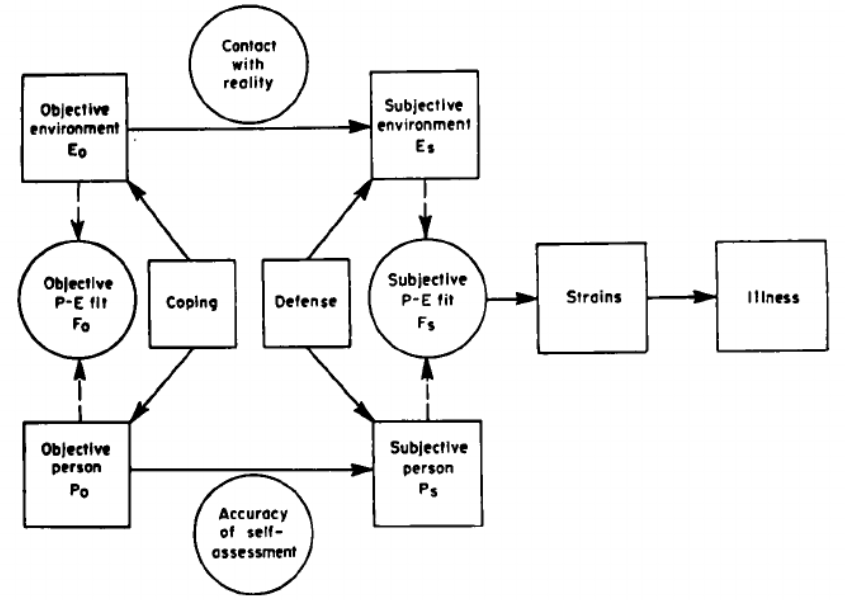
\includegraphics[width=1\textwidth]{gfx/subjektivObjektivPEFit.png}
	\caption{Hier eine Beschreibung einfügen \cite[S. 22]{edwards:2008}}
	\label{fig:personEnvironmentFit:subjektivObjektiv:abb1}
\end{figure}
\\
\textcite{copingAndAdaption:1974} betonten die Wichtigkeit, alle vier Subjekte anhand vergleichbarer Dimensionen zu messen. Dies betrachteten die Forscher als wichtige Grundlage, um aussagekräftige Ähnlichkeiten berechnen zu können. In ihren Untersuchungen bestimmten sie die in Abbildung \ref{fig:personEnvironmentFit:subjektivObjektiv:abb1} dargestellten Differenzwerte des objektiven \mbox{(F\textsubscript{O} = E\textsubscript{O} - P\textsubscript{O})} und des subjektiven \mbox{(F\textsubscript{S} = E\textsubscript{S} - P\textsubscript{S})} P-E Fits. Individuen streben den Wissenschaftlern zu Folge an, unerfüllte Anforderungen zu vermeiden. Dies gilt sowohl für unbefriedigte Wünsche der Person als auch überhöhte Ansprüche der Umgebung. Um solche Situationen zu vermeiden, existieren zwei Strategien. Ändert ein Mitarbeiter seine objektive Umgebung oder sein objektiv ermitteltes Selbst zur Verbesserung des objektiven P-E fits, sprechen \textcite{copingAndAdaption:1974} von Bewältigung (Coping). Ändert die Person ihre subjektive Wahrnehmung von Umgebung oder sich selbst zur Optimierung des subjektiven P-E fits, bezeichnen sie die Strategie als Verteidigung (Defense). Bei ihren Untersuchungen stellten die Forscher fest, dass der subjektive P-E Fit besonders bedeutsam für die Entstehung psychischer Belastungen und daraus resultierenden Krankheiten beim Mitarbeiter ist. Andere Werte wie der objektive P-E fit spielen dagegen nur eine untergeordnete Rolle. \\
Auch Publikationen anderer Forscher bestätigen die Einschätzung, dass der subjektive P-E fit aussagekräftiger für die Bestimmung von Ergebnissen ist, als der Objektive \cite[S. 3]{carless:2005}. Dementsprechend wird die subjektive Wahrnehmung des P-E Fits in der Literatur stärker fokussiert \cite[S. 8]{caplan:1987}\cite[S. 9]{caplan:1993}\cite[S. 16]{choi:2004}.\\
In einer auf den Erkenntnissen von \textcite{copingAndAdaption:1974} aufbauenden Arbeit kam \textcite{harrison:1978} sogar zu der Einschätzung, dass innerhalb des subjektiven P-E fits alleine der Needs-Supplies Fit Auswirkungen auf die mentale Gesundheit des Mitarbeiters hat. Ein Ungleichgewicht im Demands-Abilities Fit führe dagegen nur dann zu psychischer Belastung, wenn diese der Erfüllung des Needs-Supplies Fit schade. Als Beispiel für einen solchen Sachverhalt nennt \textcite{harrison:1978} eine performanceabhängige Gehalts-Auszahlung. Möchte ein Mitarbeiter die Bezahlung erhalten (Need), welche vom Arbeitgeber in Aussicht gestellt wird (Supply), hat aber nicht ausreichende Fähigkeiten (Abilities), um die dafür notwendigen Anforderungen (Demand) zu erfüllen, führe dies zu Unzufriedenheit. Der Grund ist jedoch nicht das unterschiedliche Niveau von Fähigkeiten und Anforderungen als solches, sondern die aus diesem Ungleichgewicht resultierende beeinträchtigte Bedürfniserfüllung des Mitarbeiters. Zu einer ähnlichen Einschätzung kommen auch \textcite[S. 1ff.]{lazarus:1978}. Diese untersuchten den durch das Zusammenwirken von Person und Umgebung entstehenden Stress. Dieser entwickelt sich den Einschätzungen der Wissenschaftler zu Folge nur, wenn das Individuum durch die Nichterfüllung von Anforderungen negative Konsequenzen befürchtet. Dabei kann es sich entweder um schädliche Folgen für die Gesundheit oder die Nichterfüllung innerer Werte und Ziele handeln. \\
Zusammenfassend lässt sich feststellen, dass zu wenig erfüllte Anforderungen in der Literatur meist eindeutig als Auslöser für negative Auswirkungen interpretiert werden \cite[S. 5]{schuler:1980}. Zu sehr erfüllte Anforderungen können dagegen unterschiedliche Folgen für Individuum und Organisation haben.

\section{Auswirkungen erhöhter Angebote}
\label{ch:personEnvironmentFit:auswirkungenErhoehterAngebote}
In der Literatur stellen \textcite{mechanismsOfJobStressAndStrain:1982} drei mögliche Auswirkungen vor, welche gegenüber den Anforderungen überhöhte Angebote annehmen können. Diese vertieften die Autoren auch in nachfolgenden Arbeiten \cite[S. 5f.]{caplan:1987}\cite{harrison:1978}(Harrison 1985). Die möglichen Auswirkungen erhöhter Angebote der Umgebung (Supplies) gegenüber den Bedürfnissen des Mitarbeiters (Needs) sind in Abbildung \ref{fig:personEnvironmentFit:auswirkungenErhoehterAngebote:abb1} dargestellt. \\
% Auch in Coping und Adaption?
\begin{figure}[h]
	\centering
	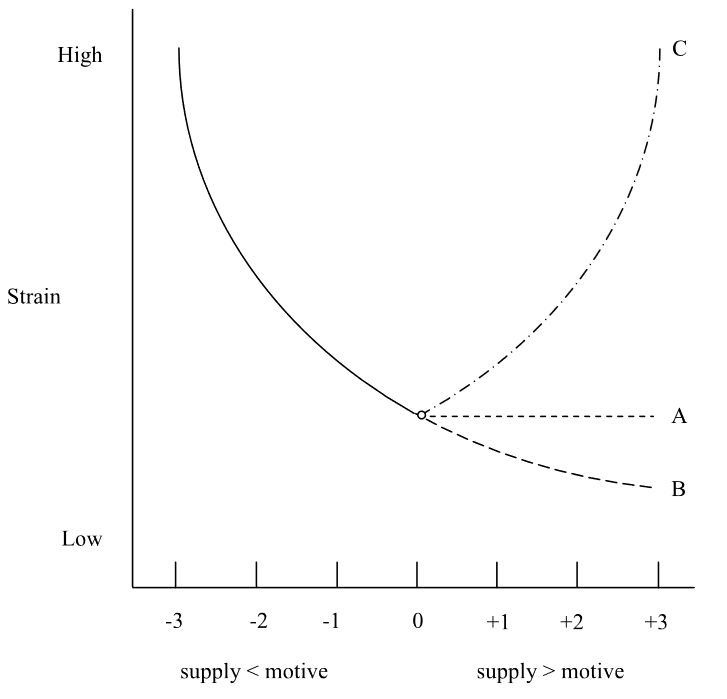
\includegraphics[width=1\textwidth]{gfx/ueberschuss_supply_motive.png}
	\caption{Hier eine Beschreibung einfügen (Beschriftung A und B tauschen) \cite[S. 23]{edwards:2008}}
	\label{fig:personEnvironmentFit:auswirkungenErhoehterAngebote:abb1}
\end{figure}
\\
An der durchgezogenen Linie in Abbildung \ref{fig:personEnvironmentFit:auswirkungenErhoehterAngebote:abb1} ist zu erkennen, dass je weniger die Bedürfnisse (Needs) einer Person erfüllt werden, die mentale Belastung (Strain) des Individuums stärker zunimmt (Quelle). Übersteigen die Angebote der Umgebung (Supply) dagegen die Bedürfnisse der Person, mündet dies in einer der drei gepunkteten Linien A, B oder C. Kurve A stellt eine asymptotische Beziehung der Überangebote zur mentalen Belastung dar. Sie tritt ein, wenn eine Person die Übererfüllung eines Bedürfnisses entweder für einen späteren Zeitpunkt aufsparen oder für die Befriedigung verwandter Motive investieren kann \cite[S. 5f.]{caplan:1987}. Dieser Sachverhalt ist beispielsweise erfüllt, wenn einer Person mehr Gehalt zusteht, als diese für die Zahlung ihrer Lebenskosten benötigt. Das überschüssige Geld könnte diese entweder für die Zahlung von Lebenshaltungskosten in den Folgemonaten aufsparen oder zusätzlich ihr mögliches Bedürfnis nach Luxusgütern befriedigen. Linie B ist U-förmig und tritt ein, wenn eine Übererfüllung eines Bedürfnisses entweder die Befriedigung dieses oder eines verwandten Motivs hemmt \cite[S. 5]{caplan:1987}. \textcite{harrison:1978} nennt hierfür das Bedürfnis einer Person nach sozialem Austausch als Beispiel, welches durch Übererfüllung deren Wunsch nach Privatsphäre verletzt. Kurve C stellt eine monotone Beziehung zur mentalen Belastung dar und tritt ein, wenn weder die Bedingungen von Kurve A noch von Kurve B zutreffen. Eine Übererfüllung dieses Bedürfnisses hat also weder positive noch negative Folgen für die Person. Ein Beispiel für eine solche Beziehung wäre ein Überangebot an vergünstigten Heißgetränken am Arbeitsplatz. Der Mitarbeiter kann die zusätzlichen Angebote nicht für einen späteren Zeitpunkt aufsparen, da diese in der Zwischenzeit abkühlen würden. Auch muss er nicht mehr trinken als er möchte, sodass keine negativen Auswirkungen auf dessen Wohlbefinden entstehen. \\
\textcite{harrison:1978} geht davon aus, dass ähnliche Beziehungen von Angeboten zu mentaler Belastung auch zu erwarten sind, wenn das Fähigkeitsniveau des Mitarbeiters (Abilities) die Anforderungen der Umgebung (Demands) übertreffen. Die entsprechend in Abbildung \ref{fig:personEnvironmentFit:auswirkungenErhoehterAngebote:abb2} dargestellten Beziehungen gelten wie in Kapitel \ref{ch:personEnvironmentFit:subjektivObjektiv} beschrieben jedoch nur, wenn das Erfüllen der Anforderungen der Umgebung zur Befriedigung innerer Werte und Ziele des Individuums beiträgt. \\
\begin{figure}[h]
	\centering
	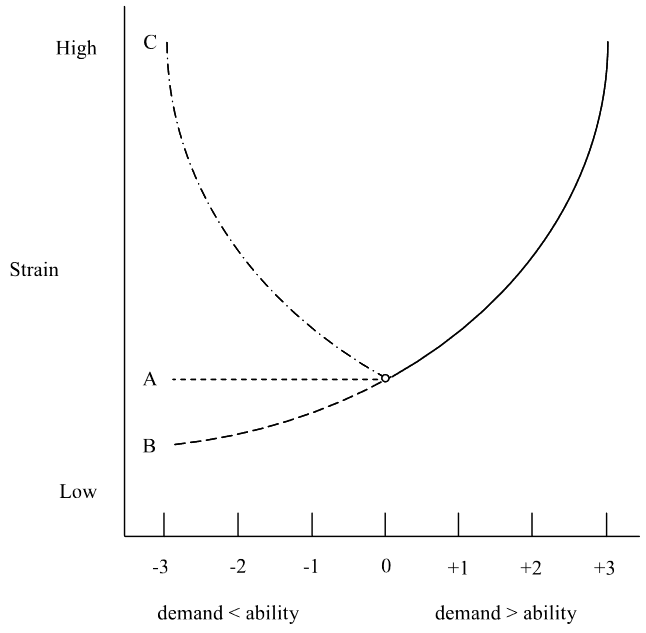
\includegraphics[width=1\textwidth]{gfx/ueberschuss_demand_abilities.png}
	\caption{Hier eine Beschreibung einfügen (Beschriftung A und B tauschen) \cite[S. 23]{edwards:2008}}
	\label{fig:personEnvironmentFit:auswirkungenErhoehterAngebote:abb2}
\end{figure}
\\
Zu ähnlichen Erkenntnissen wie \textcite{caplan:1987, copingAndAdaption:1974, harrison:1978, mechanismsOfJobStressAndStrain:1982} kommt auch \textcite{locke:1969}. Dieser betont, dass der Verlauf der Kurven in den Abbildungen zusätzlich stark von persönlichen Wichtigkeiten der Anforderungen bzw. Angebote ist. 
% Die historischen Bücher sprechen immer nur von "Männern" --> kann man daraus einfach "Menschen" machen?
% Gründungsvater ist ein englisches Zitat --> Wie zitieren?
% Wie umgehen mit den englischen Begriffen? z.B. fit, Need, Desire, etc.
\newpage
- \cite[S. 5]{caplan:1987}: Es gibt drei grundlegende Kurven, welche die Beziehung zw. PE fit der Angestellten und deren Levels von strain oder Kranksein beschreiben --> Dazu Bild im Text / Kurve A hat eine U-Form und repräsentiert die Bedingung, in welchem ein überschüssige Elemente einen Need bedrohen und ein Defizit an Elementen ein anderes Bedürfnis bedrohen kann --> bsp. Überschuss an Demand kann den Need eines Angestellten bedrohen, etwas zu erreichen und zu wenig Demand kann den Need eines Angestellten nach Stimulation bedrohen / \cite[S. 5f.]{caplan:1987}: Kurve B zeigt eine asymptotische Beziehung: Zeigt den Fall dass entweder ein Überschuss an E (Demands, Ressourcen) oder ein Überschuss an P (Needs, Abilities) das Kranksein erhöhen können --> Ein Defizit aber nicht --> Beispiel: Wenn eine P ein hohes Bedürnis nach Führung hat (Quelle) kann sie sich durch zu viele Möglichkeiten zur Entscheidungsteilhabe bedroht fühlen --> Reduzierung dieses Überschusses reduziert den Strain einer P bis zu einem Punkt, zu dem der Need erfüllt ist, nach diesem Punkt hat es nur noch wenig Strain-Reduzierende Effekte / \cite[S. 6]{caplan:1987}: Kurve C zeigt den Fall, in dem die absolute Menge einer PE fit Komponentente, relativ zu einer anderen, einen linearen Effekt auf Strain hat --> Beispiel: Je mehr Arbeit eine P relativ zur gewünschten Arbeitsmenge hat, desto mehr Strain entsteht / Es gibt auch noch weitere Kurven --> Bsp: Wenn es Intervalle gibt oder Tiefpunkt nicht exakt bei P=E liegt --> z.B. diskutiert bei Kahana 1978 oder Kulka 1979 \\
- \cite[S. 3]{edwards:1996}: Die meisten Theorien besagen, dass Strain zunimmt wenn S gegenüber V zu kurz kommt (Quellen), sind aber zweideutig bei einem Überschuss an S --> Harrison 1978 identifiziert 4 unabhängige Prozesse --> Erste zwei Prozesse geben an, dass ein Überschuss an S den Strain weiter reduziert. Erster wird als "Conservation" bezeichnet und tritt auf, wenn der Überschuss einbehalten werden kann, um den Fokuswert zu einem späteren Zeitpunkt zu befriedigen, z.B. angesammelte Urlaubstage oder überschüssiges Gehalt; 2. "Carryover": Überschuss von einem S hilft andere V zu erfüllen --> Tritt für V auf, die instrumentell verwandt sind, z.B. wenn ein Überschuss an Autonomie die Person dazu befähigt, gewünschte Veränderungen an der Arbeit vorzunehmen; Sowohl Conservation als auch Carryover zeigen eine monotone Beziehung zwischen S-V fit und Strain --> Strain nimmt weiter ab, wenn S V übersteigen / Die verbleibenden beiden Prozesse geben an, dass ein Überschuss an S den Strain erhöht: Erstes wird "depletion" genannt und tritt auf, wenn ein Überschuss an S die zukünftige Erfüllung von V auf der Fokusdimension verhindert --> z.B. Zu viel Unterstützung der Führungskraft zu einem bestimmten Zeitpunkt kann seine Unterstützung zu einem späteren Zeitpunkt ausschließen; 2. ist "Interference" --> \cite[S. 4]{edwards:1996}: Überschuss an S auf einer Dimension verhindert V-Erfüllung auf anderen Dimensionen --> z.B. Überschuss an Kontakt mit Mitarbeitern hindert das Verlangen nach Privatsphäre (Harrison 1978) --> Beide Prozesse zeigen eine gekrümmte Beziehung zw. Strain , sodass ein perfekter S-V fit optimal ist (und zu minimalem Strain führt) \\
- \cite[S. 6]{edwards:1996}: Die meisten Theorien besagen, dass Strain zunimmt wenn wahrgenommen wird, dass Demands zu hoch sind; Unterschiedliche Theorien was passiert, wenn Abilities zu hoch sind --> Ein Ansatz ist die Ansätze von Carryover, Conservation, etc. auch hier anzuwenden \\

- \cite[S. 9]{edwards:1996}: Es sind auch Sonderfälle möglich, z.B. wenn ein Überschuss an Demands den Value einer P erfüllt, sich selbst weiterzuentwickeln, dann kann der Strain trotzdem sinken \\
- \cite[S. 4]{edwards:1990}: Unterschiedliche Outcomes werden in verschiedenen Arbeiten diskutiert, z.B. Wenn Angebote der Umgebung von den individuellen Werten abweichen, entsteht Unzufriedenheit bei \textcite{locke:1969} / Im Gegensatz dazu: Übersteigen die Anforderungen der Umgebung die persönlichen Fähigkeiten, werden laut \textcite{theoryOfBehaviorInOrganizations:1980} Leistungseinbußen (Performanceeinbußen) wahrscheinlich \\
- \cite[S. 21]{edwards:2008}: Es gibt unterschiedliche Theorien wie es sich aber verhält, wenn die Supplies die Motive übersteigen --> Dann kann Strain zunehmen, abnehmen oder konstant bleiben --> Hängt davon ab, welche Auswirkungen die Übersteigung auf das Motiv oder andere Motive hat; Wenn das Überangebot nicht auf andere Motive angewendet werden kann oder für das Motiv nicht haltbar gemacht werden kann, dann sollte der NS-fit eine asymptotische Beziehung zum Strain haben (Kurve A); Wenn die übersteigenden Supplies zurückgehalten werden oder Motive anderer Dimensionen damit erfüllen können, sollte die monotone Beziehung von Kurve B entsteht --> Beispiel: Mehr Gehalt kann in Zukunft für Luxusgüter oder Dienstleistungen ausgegeben werden; Es entsteht eine U-Kurve, wen der NS fit andere Dimensionen oder dieselbe Dimension hemmt (Kurve C) \\
- \cite[S. 22f.]{edwards:2008}: Ein Ähnliches Verhalten stellen verschiedene (Quellen) auch beim demand-abilities fit fest --> (Aber nur, wenn DA misfit dazu führt, dass die Nichterfüllung der Anforderung den Erhalt von gewünschten Supplies hemmt)--> Wenn Demand größer als Abilities sind, entsteht Strain; Ist es umgekehrt, kommt es darauf an, wie die Kurve aussieht \\
- \cite[S. 21]{edwards:2008}: Weitere Arbeiten haben dieses Modell danach diskutiert (Quellen) --> Wie sich der Needs-Supply fit verhält, wird in mehren Arbeiten behandelt --> Alle sind sich einig, dass Strain zunimmt, wenn die Supplies des Environments die Needs der Person nicht erfüllen; Es gibt unterschiedliche Theorien wie es sich aber verhält, wenn die Supplies die Motive übersteigen --> Dann kann Strain zunehmen, abnehmen oder konstant bleiben --> Hängt davon ab, welche Auswirkungen die Übersteigung auf das Motiv oder andere Motive hat; Wenn das Überangebot nicht auf andere Motive angewendet werden kann oder für das Motiv nicht haltbar gemacht werden kann, dann sollte der NS-fit eine asymptotische Beziehung zum Strain haben (Kurve A); Wenn die übersteigenden Supplies zurückgehalten werden oder Motive anderer Dimensionen damit erfüllen können, sollte die monotone Beziehung von Kurve B entstehtn --> Beispiel: Mehr Gehalt kann in Zukunft für Luxusgüter oder Dienstleistungen ausgegeben werden; Es entsteht eine U-Kurve, wen der NS fit andere Dimensionen oder dieselbe Dimension hemmt (Kurve C) \\
- \cite[S. 22f.]{edwards:2008}: Ein Ähnliches Verhalten stellen verschiedene (Quellen) auch beim demand-abilities fit fest --> (Aber nur, wenn DA misfit dazu führt, dass die Nichterfüllung der Anforderung den Erhalt von gewünschten Supplies hemmt)--> Wenn Demand größer als Abilities sind, entsteht Strain; Ist es umgekehrt, kommt es darauf an, wie die Kurve aussieht \\
- \cite[S. 24]{edwards:2008}: Außerdem hat Harrison die Effekte des P-E fits auf den organisationalen Strain untersucht, welcher sich auf Probleme der Funktionsweise , welche die Produktivität und das Überleben der Organisation verhindern --> Organisationaler strain entsteht, wenn die Fähigkeiten der Angestellten unzureichend sind, um die Rollen-Anforderungen zu erfüllen / Harrison 1985 S. 42 stellt fest (Zitat), dass das erfüllen der Needs und Values fundamental für das weitere Funtionieren und existieren des Individuums genauso wie das erfüllen der Rollenanforderung fundamental für das funktionieren und existieren der Organisation ist --> In Sonderfällen kann aber auch ein N-S fit zu organisationalem Strain führen / Beziehung zw. D-A Misfit und organisationalem Strain kann laut Harrison 1985 wie in Figur 4.6 betrachtet werden --> Org. strain nimmt zu, wenn die Anforderungen die Abilities übersteigen, aber bleibt konstant, nimmt ab/zu wenn die Abilities die Demands übersteigen \\

\section{Wichtigkeiten}
\label{ch:personEnvironmentFit:wichtigkeiten}
- \cite[S. 23f.]{edwards:2008}: Harrison 1985 betrachtete, wie Wichtigkeit die Auswirkungen des P-E fits beeinflusst --> Schlägt vor (Harrison 1985, S. 38), wenn man einen P-E fit über mehrere Dimensionen macht könnte man die Wichtigkeit jeder Dimension in die Formel integrieren , die die Diskrepanz jeder P-E fit Dimension mit der Wichtigkeit dieser Dimension multipliziert \\
- \cite[S. 9]{edwards:1996}: Laut Caplan 1987 wurden verschiedene Variablen als potentielle Moderatoren des Effektes von SV fit und DA fit auf Strain --> Eine gemeinsame Variable bei SV und DA ist Wichtigkeit --> \cite[S. 10]{edwards:1996}: Es wird vermutet, dass Wichtigkeit die Effekte von SV und DA fit auf Strain intensiviert, sodass ein Misfit auf wichtigeren Dimensionen zu größerem Strain als ein Misfit auf weniger wichtigen Dimensionen führt (Quellen)\\
- \cite[S. 10]{edwards:1996}: Obwohl die Wichtigkeit die Beziehung zwischen SV und DA zu Strain moderieren, unterschiedet sich der unterliegende psychologische Prozess zwischen SV und DA fit --> Bei SV fit zeigt der moderierende Effekt der Wichtigkeit die Prämisse, dass ein Missfit ist schädlicher für die stark gehaltenen Values (Quellen); Beim DA-fit basiert die wichtigkeits-Moderation auf dem Grad zu welchem der Misfit zu wichtigen Konsequenzen führt, d.h. solche welche beinhalten substantielle Rewards oder Kosten für die Person (Quellen) --> P evaluiert, ob die Konsequenzen begehrenswert oder nicht begehrenswert sind --> Ähnlich dem Bewertungsprozess bei SV; Der DA misfit wird als wichtig angesehen, wenn er zu einem SV misfit auf anderen Dimensionen führt --> Diese Korrespondenz zw. SV und DA zeigt, dass ein DA misfit einen SV fit nicht nur verhindern kann wenn Abilities Demands übersteigen, sondern auch wenn Demands Abilities übersteigen \\
- \cite[S. 20f.]{edwards:2008}: Schon \textcite{copingAndAdaption:1974} sagten dass man Wichtigkeiten verwenden sollte. Sagten aber nicht wie.


\section{Perfekter Fit}
\label{ch:personEnvironmentFit:perfekterFit}
- \cite[S. 4]{edwards:2004}: Kristof 1996, S. 6 stellt fest: "Der optimale P-O fit ist erreicht, wenn jeder Need einer Entität ist erfüllt durch einen anderen und sie teilen dieselben grundlegenden Charakteristiken" \\
- \cite[S. 23]{edwards:2008}: Es gibt auch Erweiterungen des Frameworks, die Minima an anderen Punkten als dem P-E fit haben --> Caplan 1983 S. 39 sagt z.B. dass der meist emotional zufriedenstellenste Punkt so liegt, dass er eine kleine Herausforderung generiert. / Es gibt noch weitere Erweiterungen, z.B. wie Vergangenheit und Zukunft den Fit beeinflussen könnten \\
- \cite[S. 6]{caplan:1987}: Dass der Tiefpunkt nicht bei P=E liegt, wurde bei Kobasa\&Puccetti 1983 diskutiert)


\section{Skalen}
\label{ch:personEnvironmentFit:skalen}
- \cite[S. 14]{caplan:1987}: Es gibt bei Messungen von P und E die Bedenken, dass diese mit Elementen des anderen verunreinigt sind --> ist insbesondere Möglich, wenn Antwortskalen mit relativen Quantitäten arbeiten z.B. Arbeitsbelastung auf einer Skala von 1 (keine) bis 5 (eine Menge) eher als mit absoluten Quantitätn (z.B.  Anzahl Bücher) --> Relative Bewertung von E-Demands wie "sehr viel" kann sich auf "Im Vergleich zu gestern", "Im Vergleich zu anderen Angestellten", etc. beziehen --> Deshalb sollten keine relativen Antwortskalen verwendet werden  \\
- \cite[S. 5]{edwards:1993}: French et al 1982 haben Supplies und Preferences durch Itempaare gemessen --> Beispiel für Itempaar: "Wie viel Arbeitslast hast du?" und "Wie viel Arbeitslast würdest du gerne haben?" --> Antwortskalen reichten von "sehr wenig (1)" bis "sehr viel (5)" \\
- \cite[S. 5]{edwards:2008}: Dann können noch unterschiedliche Einheiten zur Konzeption von P und E verwendet werden --> Needs können z.B. über Einheiten oder Wichtigkeiten ausgedrückt werden --> Diese Unterscheidung hat wichtige Implikationen für die Theorien des N-S fits (Quellen) \\
- \cite[S. 8]{edwards:1990}: Messung der P und E Komponenten sollte vergleichbar sind --> Heißt: Sollten dieselbe theoretische Dimension haben --> \textcite{copingAndAdaption:1974} sagen, dass vergleichbare Messungen notwendig für Differenz-Berechnung sind --> Das ist laut \textcite{jobDemandsAndWorkerHealth:1975} die meistverwendete Prozedur in der P-E fit Forschung --> Differenzberechnungen werden meist verschiedenen Transformationen ausgesetzt, um den Punkt des 'Perfect Fit' zu bestimmen \textcite{jobDemandsAndWorkerHealth:1975} / Wenn diese Prozeduren genutzt werden, müssen die P und E Messungen nicht nur vergleichbar sein, sondern auch noch denselben Nullpunkt teilen --> sonst ist die Bestimmung des Punktes bedeutungslos \\
- \cite[S. 8]{edwards:1990}: Zweitens: Fragebögen, welche zur Messung der P und E Komponenten genutzt werden --> Sowohl bei SV als auch DA sind Fragebögen bzgl. E einfacher --> S-Fragebögen sollten fragen wie sehr das Attribut vorhanden ist, wohingegen D-Fragebögen sollten das Level (Höhe) der Demands erfragen, die mit einem betrachteten Attribut verbunden sind (vgl. \textcite{jobDemandsAndWorkerHealth:1975})/ Fragebögen zu P sind komplexer: Zu V gibt es zwei Möglichkeiten: Einmal zu erfragen, zu welchem Level die Attribute erfüllt sein sollen (\textcite{jobDemandsAndWorkerHealth:1975}) oder die Wichtigkeit der Attribute (\textcite{workAdjustment:1964}) --> Theoretische Diskussionen ergeben, dass der erste Ansatz eher für die Diskrepanz-Form und der zweite für die Interaktive Form geeignet ist (\textcite{copingAndAdaption:1974} und mehr Quellen) --> Es gibt auch Studien, die es anders bzgl. Diskrepanz machen (z.B. V durch Wichtigkeiten messen) oder manche Studien der interaktiven FOrm messen V in Desires --> Ergebnis: Ergebnisse dieser Studien lieern keine klare Interpretation über die grundlegenden Priznzipien des P-E fits / Für A veranschlagen Fragebögen oft ein Selbstassement der Fähigkeiten  oder indirekte Indikatoren der Fähigkeiten wie z.B. Bildung (\textcite{jobDemandsAndWorkerHealth:1975}) --> Vorteil des ersten Ansatzes: Man kann besser das Konstrukt messen, das einen tatsächlich interessiert, dafür ist der Ansatz anfällig für eine Antwortverzerrung durch soziale Erwünschtheit (social desirability response bias) --> Dieser Bias kann durch die zweite Methode vermieden werden, bietet aber eine weniger direkte Messung des Konstrukes, das einen interessiert --> Gibt keine klare Lösung, aber man sollte die Trade-Offs im Hinterkopf behalten \\
- \cite[S. 8f.]{edwards:1990}: Drittes Problem beachtet die Anzahl an fit-Dimensionen, die in die Studie eingebunden werden / Manche Studien (Quellen) verwenden nur eine Dimension / Sogar die systematischsten Untersuchungen zur Zeit von \cite{copingAndAdaption:1974} und \cite{mechanismsOfJobStressAndStrain:1982} enthalten nur acht Dimensionen des Fits / Wenn es nur wenige Dimensionen gibt, haben solche Studien zwei Nachteile --> 1. Wenn man annimmt, dass eine Inkongruenz über mehrere Dimensionen den strain stärker beeinflusst, vernachlässigen diese Studien notwendigerweise relevante Bestimmungsgrößen von Strain; 2. Diese Studien bieten nur limitierte Informationen über den P-E fit als generelles Konstrukt / Übergeordnete Ansätze involvieren umfassende Messungen von Person und Environment, um Indizes des fits zu bestimmen --> z.B. haben viele Studien zur Jobzufriedenheit den Work Values Inventory verwendet, um Indizes entlang von 15 Dimensionen zu bestimmen (Quellen genannt); Alternativ kann man auch Arbeitnehmer interviewn, um Job-relevante Aktivitäten und Konstrukt-korrespondierende Indizes des Fitszu erhalten --> Beide Prozeduren werden eine Einschätzung des fits bieten und sollten wenn möglich implementiert werden

\section{Berechnung}
\label{ch:personEnvironmentFit:berechnung}
- \cite[S. 1f.]{caplan:1993}: (French 1963) hielt eine Rede, in welcher er ein neues Programm für interdisziplinäre Forschung beschrieb, bekannt als Mental Health and Industry Program und heute als das Social Environment and Health Program am Institut für Sozialforschung (ISR) --> Dieses Programm generierte einige der ersten Tests der PE fit Theorie(Quellen) und einen großen Datensatz auf PE fit und Wohlbefinden von mehr als 2000 Angestellten und 23 Berufsgruppen --> Dieser diente auch für nachfolgende Tests als Ressource für Tests zur PE fit Theorie (z.B. bei \textcite{edwards:1993}) / French unterstrich in seiner Rede die Wichtigkeit der Messung von P und E entlang entsprechender Dimensionen / French beschrieb ein programmatisches Modell, dass besagt, dass Charakteristiken von P und E einen breiten Bereich von Antworten wie Verhalten, Stimmung, physische Gesundheit --> Von all diesen Reaktionen wurde angenommen, dass sie die physikalische und mentale Gesundheit beeinflussen --> Um die breiten Reaktionen zu untersuchen, stellte French Forscher verschiedener Disziplinen u.a. Epidemiologen, Physiker, Verhaltenspsychologen, etc. ein / \cite[S. 4]{caplan:1993}: Untersuchten die Verbindung zwischen Arbeitsbedingungen und Wohlbefinden / Datensatz stammt von Caplan,  Cobb,  French,  Harrison und Pinneau (1980) \\- \cite[S. 11]{caplan:1993}: Die meisten Arbeiten betrachten den PE fit eher als einen unabhängige Variable als einen Outcome (Gibt ein paar Ausnahmen; Hier mit Quellen) \\
- \cite[S. 15f.]{caplan:1993}: Edwards schlägt eine generelle Prozudur vor, die es erlaubt die Eignung von Bedingungen und Annahmen zu bestimmen --> Prozedur erlaubt die Beziehung zwischen outcome und Kongruenz auf drei Dimensionen (Bild-->zu sehen sind die Rohdaten von Caplan et al 1980) --> Dabei ist die abhängige Variable vertikal / \cite[S. 16]{caplan:1993}: Ansatz von Edwards: Statt einen Differenz-Wert zu berechnen, nimmt man die Regressionsgleichung der Modelle (z.B. von absoluter oder algebraischer Differenz) --> Dann bestimmt man Anteil der erklärten Varianz (??)\\
- \cite[S. 2]{edwards:1993}: Die P-E fit Theorie stellt drei hypothetische Beziehungen zwischen fit und strain vor --> Sind verkörpert in den five fit Messungen genutzt von (French) und (Caplan) / 1. Einfachste Messung genannt "fit" besteht aus der algebraischen Differenz zwischen E und P (E-P) --> Zeigt eine monotone Beziehung zum Strain --> Diese Beziehung wird erwartet, wenn z.B. Strain nicht nur abnimmt wenn S zu Motiven zunimmt sondern auch weiter abnimmt, wenn S übersteigt und kann auf andere Motive angewendet werden oder für spätere Verwendung zurückgehalten werden; Zwei Messungen, genannt "deficiency" (E-P für E <= P, 0 für E>P) und "excess" (E-P für E>=P, 0 für E<P) zur Darstellung von asymptotischen Beziehungen (Anmerkung für mich: Asymptotische Beziehung gab es auch bei \cite{edwards:1996}) zu Strain; Defiency repräsentiert eine negative Beziehung zu Strain nur wenn E ist kleiner als P --> Zunehmende S reduzieren den Strain bis zu einem Punkt an Zufriedenheit und haben nur noch wenig Effekt danach; Im Gegensatz dazu excess drückt eine positive Beziehung zum strain aus, nur wenn E größer ist als P --> Demands erhöhen Strain, wenn sie Abilities übersteigen, aber nciht wenn sie kleiner sind als Abilities / Zwei Messungen: "poor fit" (|E-P|) und die "squared difference" ((E-P)\^2) (hier genannt "fit squared") zeigen eine gekrümmte (curvilinear) Beziehung zum Strain --> Diese Beziehungen werden erwartet, wenn entweder übersteigen oder inadäquate S oder D sind schädlich, z.B. wenn zu viel Job-Komplexität zu einer Überlastung aber zu wenig zu Langeweile führt / Anm: Bilder zu allen Beziehungen vorhanden \\
- \cite[S. 2]{edwards:1993}: Es gibt viele Probleme an den 5 Messungen von Caplan und French (Quellen) --> Liegt an der Verwendung von Differenz-Berechnungen --> Es folgt Kritik dazu --> Probelme mit den fit Messungen können durch andere von Edwards beschriebenen Prozeduren überwunden werden --> Edwards führt in diesem Paper die Forschungen von French et al 1982 erneut aus und wendet seine empfohlenen Berechnungen darauf an --> \cite[S. 19]{edwards:1993}: Ergebnisse: 1. fit Messungen, die E und P in einen Wert zusammenrechnen sollten zugunsten von Polyomialgleichungen, welche E und P und geeignete Terme höherer Ordnung enthalten, aufgegeben werden (Quellen) / Edwards Studie demonstrierte, dass fit Messungen zu mehrdeutigen Ergebnissen führen, die separaten Beziehungen von E und P mit strain durcheinander bringen, einen sehr restriktiven Satz von Beschränkungen auferlegen, die selten unterstützt werden und reduzieren die inhärente dreidimensionale Beziehung zwischen E, P und strain auf zwei Dimensionen / \cite[S. 20]{edwards:1993}: Edwards (Quelle) Prozedur vermied diese Probleme und zeigte in den meisten Fällen, dass die Beziehung zwischen E, P und strain konnte nicht adäquat von den fit Messungen von French et al 1982 repräsentiert werden --> Grund: Diese Prozedur nutze Gleichungen, welche Fit-Messungen subsummieren, dies eliminierte die Notwendigkeit für diese Messungen und erlaubte darüber hinaus die Mesung von einer breiteren Rand von Oberflächen bezogen auf E und P zu strain --> Weitere Punkte (nachlesen) \\
- \cite[S. 2]{edwards:1990}: Sinn seines Papers: Viele Studien, die P-E fit bezüglich Stress untersuchen, sind mit ernsten theoretischen und methodischen Problemen geplagt, welche die Aussagekraft der Ergebnisse schmälern \\
- \cite[S. 3]{edwards:1990}: Dieses Paper fokussiert auf Probleme, die bei anderen Papern bzgl. Stress aufgetreten sind --> lässt sich aber auch auf andere Bereiche übertragen \\
- \cite[S. 7]{edwards:1990}: Es gibt zwei wichtige methodische Probleme in den P-E fit Studien bzgl. Stress: Erste bezieht sich auf die Messung er P und E Komponenten; Zweite betrachtet die Analyse der Beziehung zw. P E und strain \\
- \cite[S. 9]{edwards:1990}: Hier treten die größten Probleme auf / Die meisten Arbeiten bei der Diskrepanz-Form operationalisieren den Fit als algebraische Distanz (oder einer Transformation davon) zwischen vergleichbaren P und E Komponenten --> Ansatz erscheint intuitiv, die Verwendung von Differenz-Werten wurde aber stark kritisiert (einige Quellen) --> Ein Differenz-Score ist eine einfache Linearkombination seiner Komponenten --> \\
DAS NOCHMAL ANSEHEN MIT LÖSUNGSVORSCHLÄGEN \\
- \cite[S. 55]{edwards:2008}: Laut Edwards 1994 ist es das wahrscheinlich größte Problem Differenz-Werte und Profil-Ähnlichkeits-Indizes zu verwenden, um den P-E fit als eine einzige Variable auszudrücken --> Die Verwendung solcher Variablen wird oft auf theoretische Überlegungen zurückgeführt, z.B. könnte eine Theorie vorhersagen, dass der PE fit positiv mit einem Ergebnis zusammenhängt und als Reaktion wird ein Forscher Messungen von P und E zu einem Differnzwert zusammenfassung, um den P-E fit zu repräsentieren und den Wert mit der Messung eines OUtcomes korrelieren --> \cite[S. 56]{edwards:2008}: Geht nicht weiter darauf ein wurde in anderen (Quellen) schon behandelt --> Edwards macht sich eher Sorgen, dass die Berufung auf die Theorie, um die Verwendung von Differenzwerten und Profilähnlichkeitsindizes zu rechtfertigen, fehlgeleitet ist, da dies voraussetzt, dass die Theorie korrekt ist und sie von einer Überprüfung abschirmt --> Beispiel: Eine Theorie besagt, dass die absolute Differenz zwischen NS zu Zufriedenheit führt. Dann sollte nicht die Korrelation zwischen der absoluten Differenz zw. NS mit Zufriedenheit geprüft werden, sondern man sollte die Funktionsform testen, welche die absolute Differenz darstellen soll --> Diese Funktionsform sollte als zu empirisch zu testende Hypothese betrachtet werden und nicht als Annahme, die den Daten aufgezwungen wird --> ??? \\
- \cite[S. 7]{su:2015}: Verwendung von fit-Indizes ist wegen der Einfachheit des Kongruenzwertesn sehr beliebt in der Karriere-Entwicklungsforschung --> Kritisiert von Edwards --> Alternativer Ansatz von Edwards (1994, 2002): Nutzung von polynominaler Regression --> Basiert auf der Prämisse, dass P und E Messungen verschiedene Konstrukte sind und dass die funktionale Form sollte eher empirisch getestet werden als ein fit-Index angenommen zu werden; Laut Edwards sind die Gleichungen generalisierte Formen des fit-Indexes ohne ungewollte Annahmen über die Koeffizienten der Komponenten; Mit diesem Ansatz hat Edwards den Datensatz von French, Caplan und Harrison (1982) erneut analysiert und zeigte, dass er den Anteil erklärter Varianz mehr als verdoppeln konnte \\
- In \textcite{edwards:1991} werden sehr viele Methoden zur Verrechnung genannt \\

\section{Content von P und E Dimensionen}
\label{ch:notizen:contentVonPundEDimensionen}
- \cite[S. 6]{edwards:2007}: Dimensionen können auf einem Kontinuum von Generell bis speziell reichen --> Edwards schlägt drei Punkte vor: Global-, Domäne-, Facettenlevel der P und E Dimensionen / Beim globalen Level werden den Ähnlichkeiten als Ganzes ohne Bezug auf andere Vergleichsdimensionen miteinander verglichen --> beim Supplementary Fit genutzt --> z.B. um P und E oder P und andere P zu vergleichen (Quellen) / \cite[S. 7]{edwards:2007}: Domain-Level  isoliert breite Bereiche, aber unterscheidet keine Dimensionen innerhalb des Bereichs --> z.B. Werte, Persönlichkeit (Quellen) / Beim Facetten-Level wird die Ähnlichkeit spezifischer Dimensionen inerhalb breiter Bereiche verglichen, z.B. wenn man die demographische Ähnlichkeit nach Alter, Geschlecht, Rasse und Erziehung bestimmen will (Quellen) --> Gutes Bild dazu auf S. 10 \\
- \cite[S. 7]{edwards:2007}: Inhalt der P und E Dimensionen müssen vergleichbar sein (Quellen) --> Hat 2 Features: 1. Nominale Gleichheit: P und E werden mit denselben Begriffen beschrieben (sowohl bei SV als auch DA); 2. Skalengleichheit: Heißt, dass P und E mit derselben Metrik bewertet werden \cite{copingAndAdaption:1974} --> Wird erreicht, wenn dieselbe Antwortskala für P und E und unterschiedliche item stems (?) zur Unterscheidung von P und E verwendet werden --> Dieser Ansatz wird von Porters Need Satisfaction Questionaire (Quelle) vorgestellt --> Dort steht "Wie viel ist es jetzt" und "Wie viel sollte es sein"

\section{Job Zufriedenheit}
\label{ch:notizen:jobZufriedenheit}
- \cite[S. 9]{edwards:2008}: Theorien der Job-Zufriedenheit basieren auf der Prämisse, dass Job-Zufriedenheit aus dem Vergleich zwischen was ein Job bietet und was ein Angestellter benötigt, will oder verlangt vom Job (Quellen) --> Dieser Vergleich korrespondiert mit dem N-S fit in der P-E fit Literatur \\
- \cite[S. 10]{edwards:2008}: Katzell (Quelle) entwickelte ein theoretisches Modell, um die Beziehung zwischen Diskrepanzen in spezifischen Job-Facetten, Zufriedenheit mit Job-Facetten und insgesamter Job-Zufriedenheit zu erklären --> Katzell definierte Job Zufriedenheit als einen "Affekt oder Grundton", der mit einem Job assoziiert wird, der "aus der Interaktion zwischen Arbeitnehmern und ihren Job-Ereignissen entstehen: Arbeitnehmer besitzen Werte oder Bedürfnisse und der Job ist mehr oder weniger ein Instrument Erfüllung zu bieten oder Verstärken" --> Katzell bezeichnete Job Zufriedenheit als Beeinflussung vom Vergleich von den Werten des Angestellten und dem was der Job bietet / Katzell definiert Werte als "Größenordnung eines Reizes, die ein höheres Maß an Befriedigung hervorruft als diejenige, die von anderen Größen dieser Art von Reizen hervorgerufen wird" --> Das impliziert, dass die Zufriedenheit abnimmt, wenn die Stimuli in beide Richtungen von Werten abweichen. Katzell stellt dazu fest dass, "das Ausmaß zu dem ein Stimulus eine affektive Reaktion hervorruft, die weniger als maximal angenehm ist, ist direkt proportional zur absoluten Diskrepanz zwischen der Größe des Stimulus und seinem entsprechenden Wert und umgekehrt proportional zum Wert" --> wtf --> egal, steht sowieso sehr in der Kritik \\
- \cite[S. 12]{edwards:2008}: Locke entwickelte einer der einflussreichsten Diskrepanz-Theorien zur Job-Zufriedenheit / Locke definierte Job-Zufriedenheit als "den angenehmen emotionalen Zustand, der sich aus der Einschätzung ergibt dass die eigene Arbeit das Erreichen der eigenen beruflichen Werte ermöglicht oder erleichtert" (Quelle) --> Bewertungsprozess hat nach Locke 3 Elemente: 1. Die Wahrnehmung eines bestimmten Aspektes des Jobs; 2. Impliziten oder expliziten Wertestandard; 3. bewusstes oder unbewusstes Urteil über die Beziehung (z.B. Diskrepanz) zw. der Wahrnehmung und den Werten (Quelle) / Locke definiert Werte als etwas, das eine Person subjektiv "verlangt, will oder zu erreichen anstrebt" (Quelle) und fügte hinzu, dass Werte in Bezug auf Inhalt (was will die Person?) und Intensität (oder Wichtigkeit von dem gewollten) / Locke stellte zu den Werten die Needs in Kontrast, welche er als objektive Anforderungen für Gesundheit und Überleben beschrieb --> Locke sagte, dass Werte in Bezug zu Needs stehen, sodass "die ultimative biologische Funktion der Werte des Menschen es ist, seine Handlungen und Entscheidungen so zu lenken, dass sie seine Needs befriedigen" (Quelle) --> Locke vermutet, dass die Erfüllung der Werte zu Job-Zufriedenheit führt, vorausgesetzt, dass die Werte mit den Bedürfnissen vereinbar sind / \cite[S. 12f.]{edwards:2008}: Locke unterschied auch Werte von Erwartungen --> Sind Glaubenssätze über die Zukunft --> Locke ging davon aus, dass Diskrepanz zwischen Wahrnehmung und Erwartung zu einer Überraschung führt, welche befriedigend oder unbefriedigend sein kann, abhängig davon, ob das unerwartete Ereignis gewollt (desired) ist (z.B. Lottogewinn) oder ungewünscht ist (z.B. Gefeuert Werden) / \cite[S. 13]{edwards:2008}: Locke (Quelle) formalisierte seine Perspektive durch die folgende Formel:

\begin{equation}
	S = (V_c - P)V_i
	\label{fig:formel1}
\end{equation}

S steht für die Zufriedenheit (Satisfaction),  Vc für den Wert (Value Content), P für die wahrgenommene Menge und Vi für die Wichtigkeit des Wertes (Value Importance) / Locke sagt, dass entweder die absolute oder die algebraische Differenz abhängig vom Inhalt des Wertes verwendet werden muss / Zwei Beispiele mit Geld und Temperatur (Quellen) / \cite[S. 14]{edwards:2008}: Umso wichtiger der Wert, umso steiler die Kurve \\
- \cite[S. 14]{edwards:2008}: Möchte man mehrere Job-Faketten evaluieren, kann man diese addieren, um eine insgesamte Job-Zufriedenheit zu bestimmen / Einige nachfolgende Arbeiten bauen auf Locke auf (Quellen) / \cite[S. 15]{edwards:2008}: Locke erklärte, dass die Norm für Diskrepanztheorien nicht das ist was Leute erwarten oder objektiv brauchen, sondern was sie wertschätzen (value) / Locke führte auch aus, dass Menschen Werte nutzen, um ihren Job zu bewerten wie sie ihn wahrnehmen und nicht wie er aktuell ist (kann abweichen) / Lockes Modell hat aber auch einige Schwächen: 1. Zirkulär (ggf. nochmal ansehen); 2. Formel \ref{fig:formel1} ist inkonsistent mit den Beispielen von Locke inkl. den Bildern. Insbesondere (Vc-P) indiziert, dass die Zufriedenheit abnimmt, wenn die wahrgenommene Menge relativ zur gewünschten Menge steigt --> Das ist das Gegenteil des ersten Bildes; Interpretiert man (Vc-P) als absolute Differenz, dann hätte die Funktion eine V-Form, was das Gegenteil der Funktion in Abb 2 wäre. / Auch sagt locke nicht welche der beiden Berechnungsweisen für welche Job-Facetten zu nutzen sind. Er sagt nur, dass Abb 2 für die große Mehrheit der Job-Faketten genutzt werden sollte (z.B. Task-Schwierigkeit, Reisebereitschaft, etc.) (Quelle); Auch sagt er, dass die Wendepunkte und neutralen Punkte empirisch ermittelt werden müssen (Quelle) / Es kann auch andere Formen als in den beiden Abb geben / Locke selbst (Quelle) ermittelte basierend auf einer Literaturrecherche sieben Job-Facetten, die er als relevant für die Job-Zufriedenheit erachtete --> Legt dabei aber außer beim Gehalt keine Form des Graphen fest / Auch sagt Lockes Theorie wenig über Grenzbedingungen aus

\section{Job Stress}
\label{ch:notizen:jobStress}

\subsection{McGrath}
\label{ch:notizen:jobStress:mcgrath}
- \cite[S. 16]{edwards:2008}: Konzept des P-E fit ist weit verbreitet in den Theorien des Job Stresses (Quellen); Manche Theorien fokussieren den N-S fit (Quellen), andere den D-A fit (Quellen) und andere beide gleichzeitig (\cite{mechanismsOfJobStressAndStrain:1982}) \\
- \cite[S. 16]{edwards:2008}: McGraths Modell von Stress und Performance: McGrath (Quellen) fokussiert den D-A fit. Laut McGrath (Quelle) entsteht Stress durch ein Ungleichgewicht zwischen Anforderungen des Umfeldes und den entsprechenden Fähigkeiten --> Existiert nicht objektiv, sondern wie es von der Person wahrgenommen wird; Um Stress wahrzunehmen muss er Person das Ungleichgewicht bewusst sein / Stress kann sowohl bei einer Über- als auch einer Unterbelastung entstehen / Stress tritt nur auf, wenn die Person glaubt, dass die Konsequenzen des nicht erreichens der Anforderungen wichtig sind / Stress ist ein D-A Misfit, der zunimmt umso größer die Abweichung ist / McGrath stellte die folgende Formel auf (Quelle):

\begin{equation}
	ES = C(|D-A|)
	\label{fig:formel2}
\end{equation}

- \cite[S. 16]{edwards:2008}: ES ist der erfahrene Stress (experienced stress); C sind die wahrgenommenen Konsequenzen (Consequences); D sind die wahrgenommenen Anforderungen (Demands) und A sind die wahrgenommenen Fähigkeiten (Abilities) / \cite[S. 17]{edwards:2008}: In einer Studie operationalisierte McGrath Stress als eine physikalische Erregung und fand heraus, dass diese hoch war, wenn die Differenz zwischen Anforderungen und Fähigkeiten klein war (Quelle) --> McGrath interpretierte dieses Ergebnis als ein Manifestierung von Unsicherheit basierend auf der Annahme, dass die Unsicherheit eine Aufgabe zu erfüllen zunimmt, wenn die Anforderungen und Fähigkeiten nah beieinander sind --> Annahme: Erfolg wird wahrscheinlich, wenn Fähigkeiten die Anforderungen übersteigen und Verlust wird wahrscheinlich, wenn die Anforderungen die Fähigkeiten übersteigen --> Aus dieser Schlussfolgerung passte McGrath seine Formel an:

\begin{equation}
	ES = C(K-|D-A|)
	\label{fig:formel3}
\end{equation}

- \cite[S. 17]{edwards:2008}: K ist dabei eine Konstante --> Dadurch dass |D-A| von K abgezogen wird, zeigt die Gleichung, dass Stress (bzw. Erregung) zunimmt, wenn die Lücke zwischen D und A abnimmt \\
- \cite[S. 18]{edwards:2008}: Die Definition von Stress als Erregung wird in der Stress-Literatur diskutiert (Quellen)

\section{Berufliche Kongruenz}
\label{ch:notizen:beruflicheKongruenz}
- \cite[S. 25]{edwards:2008}: Der P-E fit ist zentral für Theorien der beruflichen Kongruenz, viele davon betrachten das Match zwischen Needs, Interessen und Fähigkeiten der Person und Verstärkern und Anforderungen (verschiedene Quellen) \\
- \cite[S. 26]{edwards:2008}: Wichtigster Forscher: Holland (Mehrere Quellen) \\
- \cite[S. 26]{edwards:2008}: Berufliche Kongruenz steht auch bei Theorien zu Arbeitsanpassung im Vordergrund

\subsection{Dawis und Lofquist}
\label{ch:notizen:beruflicheKongruenz:dawisUndLofquist}
- \cite[S. 28f.]{edwards:2008}: \textcite{workAdjustment:1964} legten den Grundstein für die Theorie des "Work adjustment" --> Konzeptualisierten die Person mit Abilities und Needs / Environment wurde beschrieben durc Ability-Requirements (benötigte Anforderungen für eine zufriedenstellende Arbeitsperformance) und ein Verstärkungssystem (Spezifikationen der verstärkten Werte von Klassen von Stimulusbedingungen) (In Klammern Zitate) --> Diese P E Konstrukte wurden in zwei Typen von Korrespondenz gemappt: Eine bezieht sich auf die Ähnlichkeiten zwischen Fähigkeiten der Person und den Fähigkeits-Anforderungen der Umgebung; Die andere betrachtet die Ähnlichkeit zwischen den Bedürfnissen einer Person und dem Verstärkungssystem der Umgebung --> \textcite{workAdjustment:1964} sagen, dass man die Begriffe zur Beschreibung von Abilities und Needs auch zur Beschreibung benötigter Fähigkeiten und verfügbaren Verstärkern genutzt werden sollten, sodass vergleichbare Dimensionen vorliegen --> Proximal Outcome der Korrespondenz ist dann Zufriedenheit (Definiton: "Die Evaluation des Individuums der Stimulus-Bedingungen der Arbeitsumgebung mit Bezug auf deren Effektivität bzgl. der Verstärkung seines Verhaltens") und Zufriedenstellung ("Evaluation des Arbeitsverhaltens in Bezug auf die Qualität und Quanität der Arbeitsperformance und/oder Performance-Outcomes (Produkte, Services)") / Zitate von \cite{workAdjustment:1964}: Zufriedenheit ist eine Funktion der Korrespondenz zwischen Verstärkungssystem der Arbeitsumgebung und den Needs des Individuums, vorausgesetzt dass die Fähigkeiten des Individuums mit den Fähigkeitsanforderungen der Arbeitsumgebung korrespondieren ... Zufriedenstellung ist eine Funktion der Korresondenz zwischen den Fähigkeiten des Individuums und den Fähigkeitsanforderungen der Arbeitsumgebung, vorausgesetzt, dass die Needs des Individuums mit dem Verstärkungssystem der Arbeitsumgebung korrespondieren" / Erkenntnis: Zufriedenstellung mäßigt die Effekte von Needs-Verstärkungssystem auf Zufriedenheit und genauso mäßigt Zufriedenheit die Effekte von Fähigkeiten-Fähigkeitsanforderungs-Korresponenz auf Zufriedenstellung --> "Work adjustment" ist definiert als kombinierte Levels von Zufriedenheit und Zufriedenstellung einer Person --> \cite{workAdjustment:1964} stellten auch fest, dass Zufriedenstellung und Zufriedenheit die Wahrscheinlichkeit beeinflussen, mit welcher eine Person in einer Arbeitsumgebung bleibt oder sie verlässt \\
- \cite[S. 29ff.]{edwards:2008}: Die Theorie wurde von Dawis et al. 1968 und Lofquist und Dawis 1969 grundlegend geändert und aktualisiert von Dawis und Lofquist 1984 \\
- \cite[S. 31]{edwards:2008}: Die letzte Version (Dawis und Lofquist 1984) definiert Fähigkeiten als empirisch abgeleitete Faktoren, die spezifische Fähigkeiten umfassen, die "wiederkehrende Reaktionssequenzen sind, die dazu neigen, durch Wiederholung modifiziert und verfeinert zu werden" (Zitat) / Analog dazu sind Values Faktoren, die spezifische Needs umfassen, die definiert sind als "Das Bedürfnis eines Individuums nach einem Verstärker auf einem bestimmten Niveau der Stärke" --> Stärke ist die Wichtigkeit eines Bedürfnisses --> Ich schließe aus dem Kontext: Je größer die Stärke, desto Häufiger muss die Reaktion des Verstärkers sein; Werte sind Wichtigkeitsdimensionen als Referenzdimensionen für die Beschreibung von Needs --> Needs sind Präferenzen für Verstärker ausgedrückt als relative Wichtigkeit für jeden Verstärker für das Individuum / Definition Korrespondenz: "Harmonische Beziehung zwischen Individuum und Umgebung, Eignung des Individuums für die Umwelt und der Umwelt für das Individuum, Übereinstimmung oder Einvernehmen zwischen Individuum und Umgebung sowie eine wechselseitige und ergänzende Beziehung zwischen Individuum und Umwelt" --> Es besteht also eine wechselseitige Beziehung zwischen Individuum und Umgebung / Definitionen für Zufriedenheit und Zufriedenstellung \\
- \cite[S. 32]{edwards:2008}: Kritik von Edwards an Dawis and Lofquist: Deren Theorie definiert Person und Umgebungs-Konstrukte auf eigene Art und Weise / \cite[S. 33]{edwards:2008}:  Auch sind Bedeutungen von Zufriedenheit und Zufriedenstellung unklar dargestellt

\section{Recruiting und Selektion}
\label{ch:notizen:rekcruitingUndSelektion}
- \cite[S. 33]{edwards:2008}: P-E fit ist fundamental, wenn Menschen mit Jobs in Unternehmen gematcht werden (Quellen) / Forschung in diesem Bereich identifiziert meist das notwendige Wissen, Fertigkeiten und Fähigkeiten für einen Job, misst diese Attribute bei möglichen Angestellten und untersuchen den Zusammenhang zwischen diesen Messungen und späterer Arbeitsleistung (Performance) --> Diese Forschung adressiert nicht direkt den Fit zwischen Person und Job, weil die persönlichen Attribute nicht berücksichtigt werden (Schneider, 2001) --> Edwards betrachtet nur Theorien, die explizit den P-E fit behandeln

\subsection{Wanous Matching Modell}
\label{ch:notizen:rekcruitingUndSelektion:wanous}
- \cite[S. 34f.]{edwards:2008}: Modell von Wanous ist eine Adaption der Work Adjustment Theorie von Lofquist und Dawis 1984 / Betrachtet SV- und den DA-fit / Auch hier gibt es Reinforcers / Abilities sind definiert als "was Menschen jetzt tun können oder potentiell in der Zukunft tun können werden" (Genauso auch die Anforderungen); Needs sind definiert als "grundlegendes Streben oder Verlangen"; Im Gegensatz dazu werden Verstärker und Anforderungen nicht explizit definiert / Laut Modell führt DA fit zu Job-Performance --> Zitat: Mismatch führt bei Fähigkeiten und Job-Anforderungen führt zu schlechter Performance; Match zwischen Bedürfnissen und Verstärkern führt zu Jobzufriedenheit und Organisationalem Commitment --> Definition Jobzufriedenheit: "Match zwischen Needs einer Person und erhaltener Verstärkung durch die erledigte Arbeit"; Definition Organisationales Commitment: "Dem Match zwischen Menschlichen Needs und den Verstärkungen, die man durch die das nicht-job Klima er Organisation erhält" / Johannes: Aus Modell ist abzulesen, dass Job-Performance zu einer Reaktion beim Unternehmen führt (Feuern, .., bleiben) und Job Zufriedenheit und Commmitment zu einer Reaktion beim Mitarbeiter (Gehen, bleiben) \\
- \cite[S. 35]{edwards:2008}: Später erstellte Wanous (1992) ein neues Modell getrennt von seinem alten Modell (Meiner Ansicht nach ändert sich da aber nicht viel)

\subsection{Breaughs Person-Job Congruence Model}
\label{ch:notizen:rekcruitingUndSelektion:breaugh}
- \cite[S. 36]{edwards:2008}: Braugh entwickelte ein Modell für einen Rekruting-Prozess der die person-job Kongruenz als zentrale Komponente unterstützt --> P-J Kongruenz definiert er als "Diskrepanz zwischen den Attributen, die ein e Organisation von einem potentiellen Angestellten verlangt und den Charakteristiken die eine Person bietet und die Diskrepanz zwischen dem was die Person von der Organisation will und den Anreizen, die der Arbeitgeber bietet" --> \cite[S. 37]{edwards:2008}: (Zitate) D-A fit führt zu einem zufriedenstellenden Level an Job-Performance und ein guter fit zwischen den Wünschen der Person und den Attributen der Job-Angebote führt zu einem Gefühl der Wertsteigerung, was wiederum zu Arbeitszufriedenheit führen wird" / Nachteil nach Edwards: Beschreibt keine Metrik, mit der Person und Job verglichen werden können --> Aber es gibt ein paar Beispiele / In einer Fußnote schreibt Breaugh, dass der P-J fit sich auf die Wahrnehmung der Kongruenz zw. DA und SV bezieht (das muss ich nochmal nachprüfen) / Modell bleibt auch wage bei der Form der Beziehung zwischen Kongruenz udn Outcomes --> In einer Fußnote stellt Breaugh fest, dass für manche Organisationalen Attribute ein Individuum weder zu viel noch zu wenig von einem Attribut sucht (z.B. Reisen). Bei anderen Attributen gitl, umso mehr die Organisation bietet (z.B. Bezahlung) desto besser wird die Person den fit bewerten --> Bestimmte Attribute werden aber nicht genannt

\subsection{Werbel and Gillilands Facet Model of Fit}
\label{ch:notizen:rekcruitingUndSelektion:werbel}
- \cite[S. 37]{edwards:2008}: Werbel und Gilliland stelleten ein Faketten-Modell des P-E fits vor, welches den Auswahlprozess in Bezug auf Person-Job fit, Person-Workgroup fit und Person-Organization fit bezieht / P-J fit ist definiert als (Zitat) Kongruenz zwischen Job-Anforderungen und den benötigten Skills, Wissen und Fähigkeiten eines Job-Kandidaten --> \cite[S. 38]{edwards:2008}: Laut 
Modell führt der P-J fit zu Leistung, technischem Verständnis und Arbeitsinnovationen / Person-Workgroup fit bezieht sich auf das (Zitat) Match zwischen dem Neuangestellten und der gesamten Arbeitsgruppe (z.B. Mitarbeiter und Führungskräfte) --> P-W fit wird sowohl durch einen supplementary als auch einen complementary fit bestimmt: Supplementary, da Werte, Ziele, Persönlichkeit übereinstimmen müssen und complementary, da die Gruppe heterogene Skills, Leistungen und Netzwerke mitbringen muss, sodass (Zitat) Performance-Schwächen eines Individuums durch die Performance-Stärken eines anderen Individuums ausgeglichen werden können / P-O fit enthält einen supplementary fit und einen needs-supply fit; Supplementary fit ist beschrieben als Kompatibilität zw. dem Wertesystem der Person und der Organisation; NS fit bezieht sich auf das Match (Zitat) zwischen den Bedürfnissen des Bewerbers und dem organisationalen Belohnungssystem --> Ergebnis des Fits sind Organizational Citizenship Behaviors (OCBs), organisationale Zufriedenheit, organisationales Commitment und Bewahrung / Die Outcomes aller drei fits sind mit insgesamter Performance und organisationaler Effektivität verbunden / Kommentare von Edwards: Modell ist dahingehend bemerkenswert, dass es drei Typen von P-E Fits betrachtet und kollektiv NS und DA und supplementary fit anspricht

\section{ToDo}
\label{ch:todo}
- Manche Arbeiten unterscheiden zwar explizit zwischen subjektiven und objektiven P und E --> Ausnahme von der Regel (Edwards) --> bei SV-fit ist subjektive Wahrnehmung üblich \\
- Am Anfang Edwards Definitionen für P, E, fit und P-E fit verwenden, danach einzelne Definitionen für die Konstrukte suchen \\
- Was ist organisationales Verhalten \\
- Gliederung: Wichtigkeiten und dann sagen, dass aber auch Autoren zum Ergebnis kommen, dass DA für Individuum vollkommen egal ist --> Reinforcers --> Obwohl diese Verstärker so wichtig sind, werden sie bei der Personal-Auswahl häufig vernachlässigt (nur DA) --> Diese fehlende Beachtung von SV spiegelt sich auch in der Implementierung von Empfehlungssystemen wieder --> Switch zu RS \\
- Merke ein Konstrukt ist z.B. Demand oder Supply \\
- Es ist nicht möglich, alle Varianten und Arbeiten zu behandeln, wie geht man damit um? \\
- Interessant: Supplies werden auch als "Verstärker" für Needs betrachtet \\
- Nochmal nach den Definitionen für DA und SV bei Edwards suchen \\
- Es gibt viele Arten von Fits (PO, PJ, PW, etc.) --> Klar machen, dass hier nur PJ fokussiert wird (PW siehe Werbel; PO siehe O-Klima bzw. Schneider bei Klima) \\
- Wichtigkeit spielt vor allem beim supplementary fit eine Rolle --> Dieser wird in dieser Arbeit eher ausgeklammert, weil ich mich auf P-J fokussiere und supplementary eher verwendet wird, um zu schauen ob eine Person zu anderen Personen oder überhaupt in eine Org passt. Dennoch spielen Wichtigkeiten auch in manchen Umsetzungen des complementary fit eine Rolle. --> Wichtigkeiten \\
- Wichtigkeiten beziehen sich bei SV auf die Werte bei DA auf die Konsequenzen --> Person ist es egal, ob sie Anforderungen erfüllt --> Neues Kapitel \\
- Eigentlich ist es mir als Person nur wichtig meine eigenen Werte zu erfüllen (SV) --> D.h. "Performance" ist nur ein Nebenergebnis der SV-Erfüllung \\
- Lazarus nochmal prüfen \\

\section{Fazit}
\label{ch:fazit}
- Ob man die Anforderungen der Stelle erfüllt, ist dem Mitarbeiter eigentlich egal. Ihn interessiert es nur, ob dadurch seine Werte verstärkt/erfüllt werden. Es wäre also interessant, herauszufinden, wieso ein Mitarbeiter z.B. mehr Python anwenden würde. Mehr Gehalt wegen Data Science? Neugier für neue Sprache? Kumpel arbeitet in dieser Abteilung? ... \\
- Eigentlich müsste der Prozess des Motivations-Herausfindens dem kompletten Einstellungsprozess vorgelagert sein. Bzw. sogar dem Studium \\
- Grenze: \textcite{cable:1997} stellten fest, dass das Bauchgefühl des Interviewers besser vorhersagen kann, ob eine P zur O passt. Wenn also ein Unternehmen so klein ist, dass der "Staffer" alle Berater persönlich kennt, kann er wahrscheinlich besser zuordnen als die KI \\
- Anmerkung von mir: Während \textcite{parsons:1909} 1909 also noch davon ausging, dass alles möglichst objektiv und wissenschaftlich korrekt gemessen werden muss, gehen Psychologen heute davon aus, dass primär die subjektive Wahrnehmung eine Hauptrolle spielt \\

\shorthandon{"}